\chapter{システム構成と3Dモデルの取得}
\label{ch:system}

本章では，本論文で扱う三つの料理マニピュレーション研究に共通する基盤として，ロボットシステムの構成と，対象物および作業環境の3Dモデル取得方法を述べる．
本論文の中心は，3Dモデルを単なる形状の記録として扱うのではなく，動作生成，力学解析，および制御設計のための計算基盤として利用する点にある．
このため，各タスク実現するための詳細なアルゴリズムを述べる前に，それらの前提となる共通の計測・モデリング過程を明確にしておく必要がある．

本論文で扱うタスクは，液体を注ぐ操作，ピーラーによる食材表面に沿った皮むき操作，および切断時における食材の安定把持である．
これらは対象物の物理特性や要求される制御方式こそ異なるものの，いずれも対象物の三次元形状や作業空間の幾何情報を把握し，そこから操作に必要な量を計算するという点で共通している．
具体的には，注ぐ操作では容器内部形状から容積や液面検出に必要な情報を得る必要があり，皮むき操作では食材表面形状から軌道を生成する必要があり，切断する時の把持では食材表面上で把持点候補を生成し，把持安定性を評価する必要がある．

なお，システムの一部（ロボットアーム，ソフトウェアフレームワーク）は研究の進行に伴い変更が生じたが，3Dモデル取得・処理のアルゴリズムは全研究で一貫しており，本章後半で述べる点群処理パイプラインは制御方式こそ異なるもののに依存しない共通基盤として位置づけられる．

このような観点から，本章ではまず各研究で用いたロボットシステムを整理し，次にRGB-Dカメラを用いた多視点撮影による3Dモデル生成手順を述べる．
さらに，生成した3Dモデルから抽出される幾何情報と，各タスクにおけるその利用方法をまとめる．
最後に，3Dモデル取得の精度評価について述べ，本章で構築する基盤の妥当性を示す．



\section{ロボットシステムの構成}

本論文で扱う注ぐ動作，皮むき動作，および把持の研究では，共通の双腕ロボットシステムを用いた．
本章で述べるロボットシステムは，筆者の修士論文で構築した料理ロボットシステムを基盤としている．
本節では，まず三つの研究に共通するロボット，視覚センサ，力覚センサ，グリッパについて述べ，その後，ソフトウェア構成と各研究におけるエンドエフェクタ設計を説明する．

\subsection{ロボットシステム}

\subsubsection{双腕ロボット}

実験には，三菱重工製の7自由度マニピュレータ PA10-7C を2台用いた（図\ref{fig:robot_env}）．
両アームは卓上作業に適するよう床面から約700\,mmの高さに設置し，各アームのベース座標系の原点は各アームの底の中央に設定した．
各軸の向きはロボット前方を$x$軸，ロボットから見て左方向を$y$軸，鉛直上方を$z$軸とした．

双腕共同作業を統一的に記述するため，世界座標系を定義した．
世界座標系の原点は左アームのベース座標系と一致させ，各軸の向きも左アームのベース座標系と同様に設定した．
回転の表現には$x$-$y$-$z$軸周りのオイラー角を用い，各回転角度を$\alpha,\beta,\gamma$と表す．プラス回転方向は各回転軸に対して逆時計回りとした．

また，各アームがお互いの動作を妨害せずに共同作業を可能とするため，両アームのベース座標系間の距離を$Y$軸方向に804\,mmとした．

\begin{figure}[ht]
    \centering
    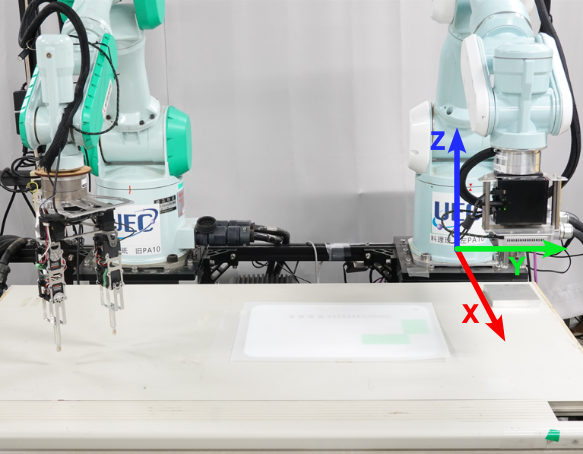
\includegraphics[width=.8\linewidth]{fig/chp3/ICRA_RobotEnv.png}
    \caption{ロボットシステムと座標系}
    \label{fig:robot_env}
\end{figure}

なお，第三研究（把持）の後半では，PA10-7C二台の故障に伴い，DENSO製VS-050へ変更した．
VS-050は6軸の垂直多関節ロボットであり，可搬質量4\,kg，位置繰り返し精度$\pm 0.02$\,mmの性能を有する．PA10-7Cと同様に双腕構成で使用し，両アームのベース座標系間の距離は$Y$軸方向に800\,mmとした．ツール座標系の定義や世界座標系の設定はPA10-7Cの場合と同様である．

\subsubsection{ツール座標系}

ツール座標系は，ロボットが操作する道具の座標系である．
道具を目的の位置・姿勢へ誘導する際，ロボットの手先座標系を直接制御するよりも，道具先端に設定した座標系を制御するほうが直感的かつ高精度な動作記述が可能となる．

PA10-7Cでは三菱重工が提供するPAライブラリを用いて手先の位置姿勢を制御する．
本研究では，ロボット手先にツールを装着した状態で各種作業を実行するため，以下のようにツール座標系を定義した．
PA10手先座標系の原点は手先フランジの中心に位置し，姿勢はベース座標系に対して$Y$軸周りに180度回転させた姿勢である．
ツール座標系の原点は装着したツールの中心（ピーラーであれば刃先，把持用エンドエフェクタであれば指先中心）に設定し，姿勢はPA10手先座標系から$Y$軸周りに180度回転させた姿勢，すなわちベース座標系と同一方向となるように定義した（図\ref{fig:tool_coordinate}）．
各種ツールに対応するため，ツール座標系の位置・姿勢はプログラム上で調整可能とした．

\begin{figure}[ht]
    \centering
    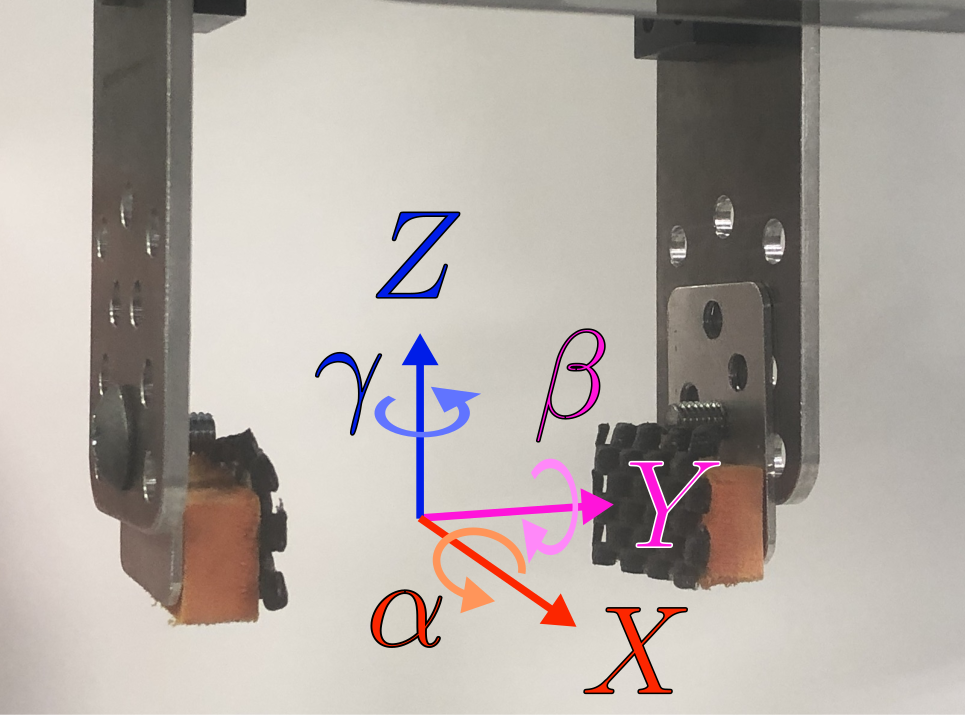
\includegraphics[width=0.7\linewidth]{fig/chp3/ToolCoordinate.png}
    \caption{ツール座標系}
    \label{fig:tool_coordinate}
\end{figure}

VS-050においても同様に，手先フランジ中心を基準としたツール座標系を定義し，ツール先端の位置姿勢を制御の基準とした．


\subsection{力覚センサ}

ロボットと対象物との接触を伴う操作を安定に実現するため，双腕の手首部には Leptrino 製の6軸力覚センサ PFS080YA501U6S を装備した（図\ref{fig:force_sensor_install}）．
このセンサはUSB経由で制御用PCに接続し，作業中に発生する力およびモーメントを計測する．

\begin{figure}[ht]
    \centering
    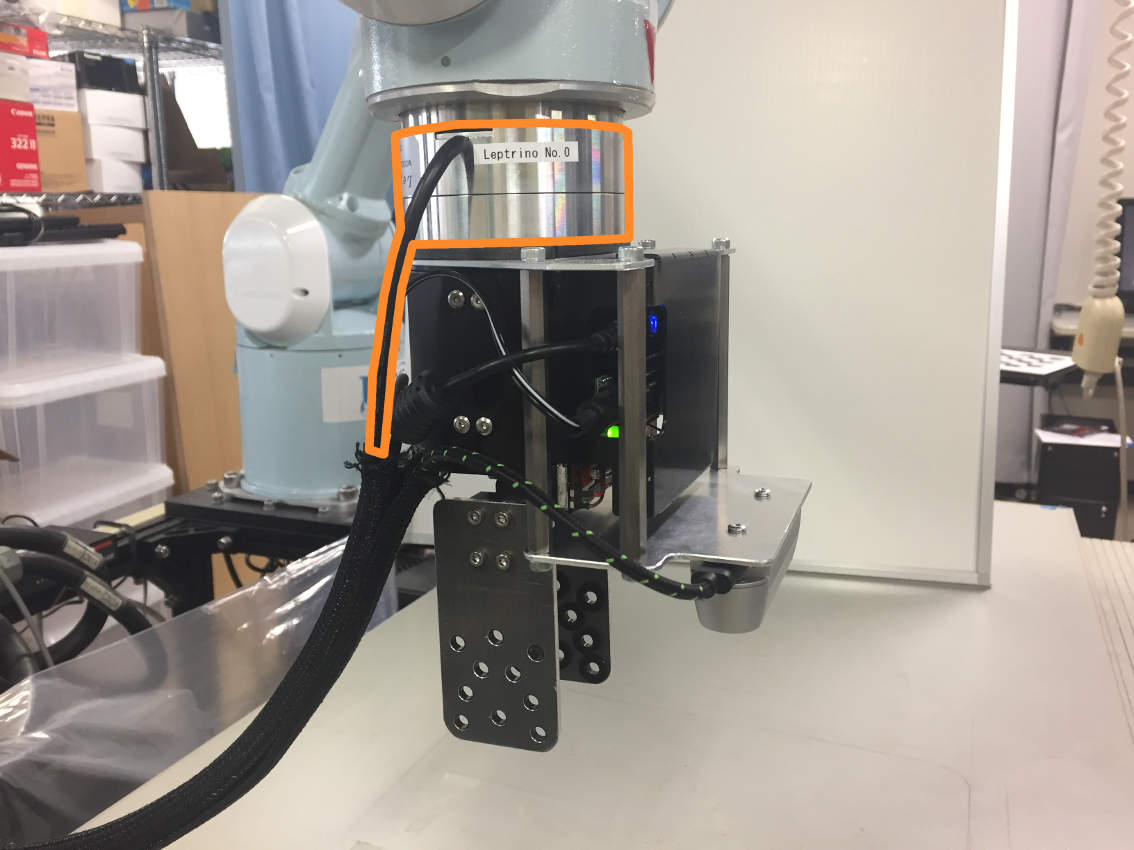
\includegraphics[width=.7\linewidth]{fig/chp3/ForceSensor.jpg}
    \caption{手首に取り付けたLeptrino製の6軸力覚センサ}
    \label{fig:force_sensor_install}
\end{figure}

本センサの性能パラメータを図\ref{fig:force_sensor_spec}に示す．
データシートに基づき，本センサの力の分解能は以下の通り計算される：

\begin{equation}
\begin{split}
\text{分解能} &= \text{定格荷重} \times \text{分解能} \\
&= 500\;\mathrm{N} \times (1 / 4000) \\
&= 0.125\;\mathrm{N}
\end{split}
\end{equation}

\begin{figure}[ht]
    \centering
    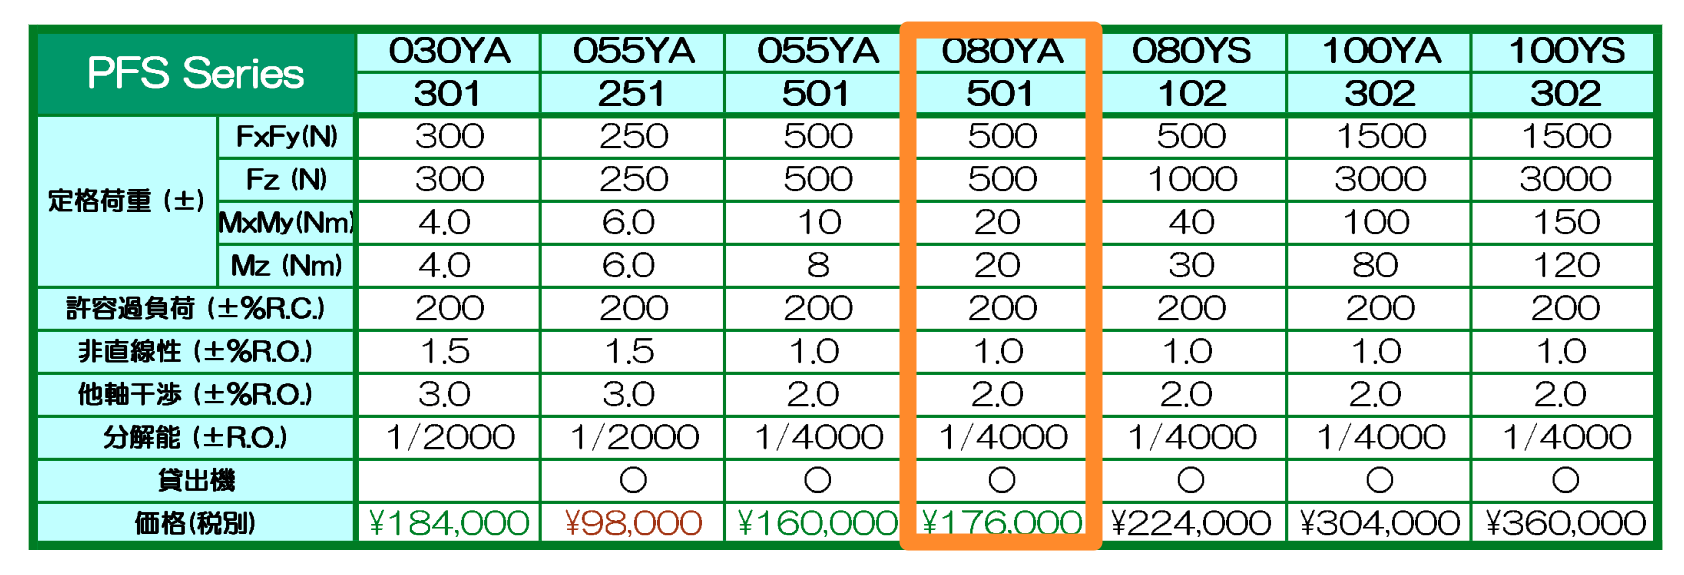
\includegraphics[width=1\linewidth]{fig/chp3/ForceSensor-performence.png}
    \caption{PFS080YA501U6Sの仕様書}
    \label{fig:force_sensor_spec}
\end{figure}

% 力覚情報は，特に工具と対象表面との接触が重要となる皮むき動作において有効であり，接触状態の確認および制御入力の設計に用いた．
% また，本論文では，3Dモデルに基づく幾何学的解析に加えて，接触に伴う力学的な情報も操作設計の一部として扱うため，力覚センサはそのための共通計測基盤として位置づけられる．
力覚情報は，皮むき動作では接触状態の監視と力フィードバック制御の入力として，把持研究では把持安定性の評価の補助情報として用いた．
このように，力覚センサは3Dモデルを補完する計測手段として，接触を伴うタスクにおいて重要な役割を担う．



\subsection{グリッパ}
力覚センサの先端には，三菱電機製の平行グリッパ1E-HM01 HANDを取り付けた（図\ref{fig:robot_gripper}）．
本グリッパの指先に取り付けられたアルミ板には，様々な姿勢でツールを装着できるように多数の穴が設けられており，各研究の要件に応じてエンドエフェクタを交換可能な構造となっている．

\begin{figure}[ht]
    \centering
    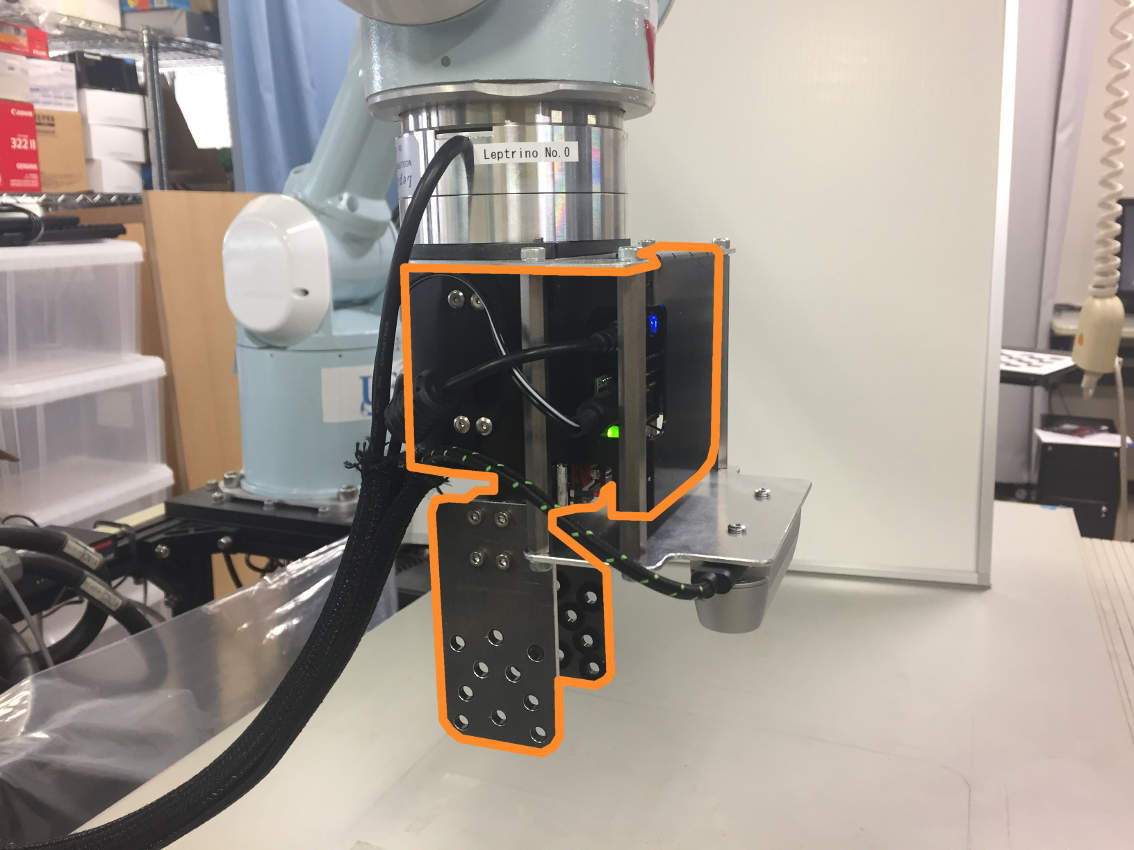
\includegraphics[width=.7\linewidth]{fig/chp3/Gripper.jpg}
    \caption{平行グリッパ（オレンジ枠内）}
    \label{fig:robot_gripper}
\end{figure}


\subsection{視覚センサ}
\label{sec:vision_sensor}

対象物および作業環境の3D情報取得には，Intel RealSense D435 を用いた．
本センサはRGB画像と深度画像を同時に取得できるRGB-Dカメラであり，容器，食材，液面，および反射を含む表面に対しても比較的安定した深度情報を取得できる．
図\ref{fig:robot_camera}のように，カメラは主としてグリッパ前面に取り付け，ロボットアームの動作により視点を変化させることで，複数視点から点群を取得した．
同時に異なる角度から点群を撮影する目的で，RealSense D435を両アームに取り付けた．

\begin{figure}[ht]
    \centering
    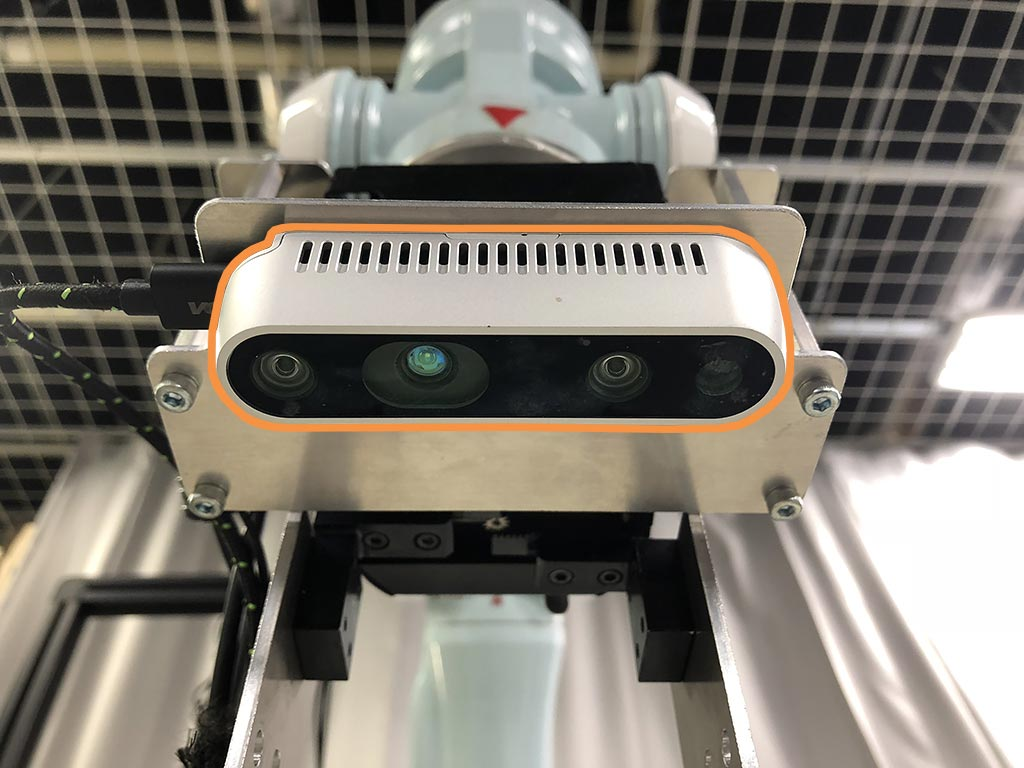
\includegraphics[width=.7\linewidth]{fig/chp3/Realsense.jpg}
    \caption{手首に取り付けたIntel RealSense D435}
    \label{fig:robot_camera}
\end{figure}

取得した点群は，各時刻におけるロボット姿勢とカメラの取り付け関係に基づいて世界座標系へ変換し，統合した3Dモデルとして利用する．
この3Dモデルは，注ぐ動作では容器内部形状の推定と容積計算に，皮むき動作では食材表面形状の取得と工具軌道生成に，切断時把持では接触候補点の生成と把持安定性評価に用いられる．


\subsection{エンドエフェクタ設計}

\subsubsection{注ぐ動作におけるエンドエフェクタ設計}

注ぐ動作では，各種容器を安定に把持し，必要に応じて持ち上げ，傾ける必要がある．
そこで，平行グリッパを基盤とし，その指先アルミ板に容器把持用のエンドエフェクタを取り付けた．
本研究では，対象容器の形状差に対応するため，2種類のエンドエフェクタを用いた．

第1のエンドエフェクタ（図\ref{fig:pour_endeffactor_1}）は，ボウルやカップのように開口縁を有する容器を対象としたものである．
平行グリッパの開口幅（最大10\,cm）のみでは把持が困難な場合を想定し，容器本体ではなく縁部を把持できるように設計した．
また，把持時の摩擦力を高めるため，接触面には小型のスポンジを取り付けた．

\begin{figure}[ht]
    \centering
    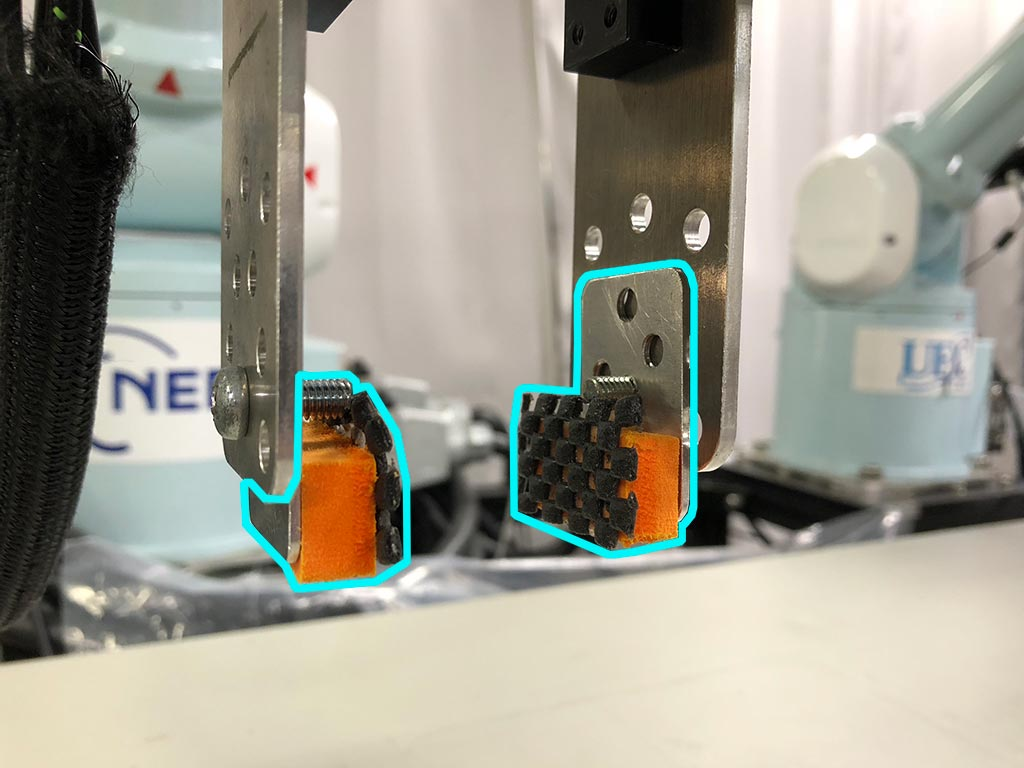
\includegraphics[width=.7\linewidth]{fig/chp3/PourEndFactor-1.jpg}
    \caption{注ぐ動作のエンドエフェクタ1}
    \label{fig:pour_endeffactor_1}
\end{figure}

第2のエンドエフェクタ（図\ref{fig:pour_endeffactor_2}）は，外形寸法が比較的小さく，グリッパ開口幅内に収まる容器を確実に把持することを目的としたものである．
こちらも把持安定性向上のため，接触面に薄いスポンジを取り付けた．
このように，注ぐ動作におけるエンドエフェクタ設計では，容器形状の多様性に対して，把持を切り替えられることを重視した．

\begin{figure}[ht]
    \centering
    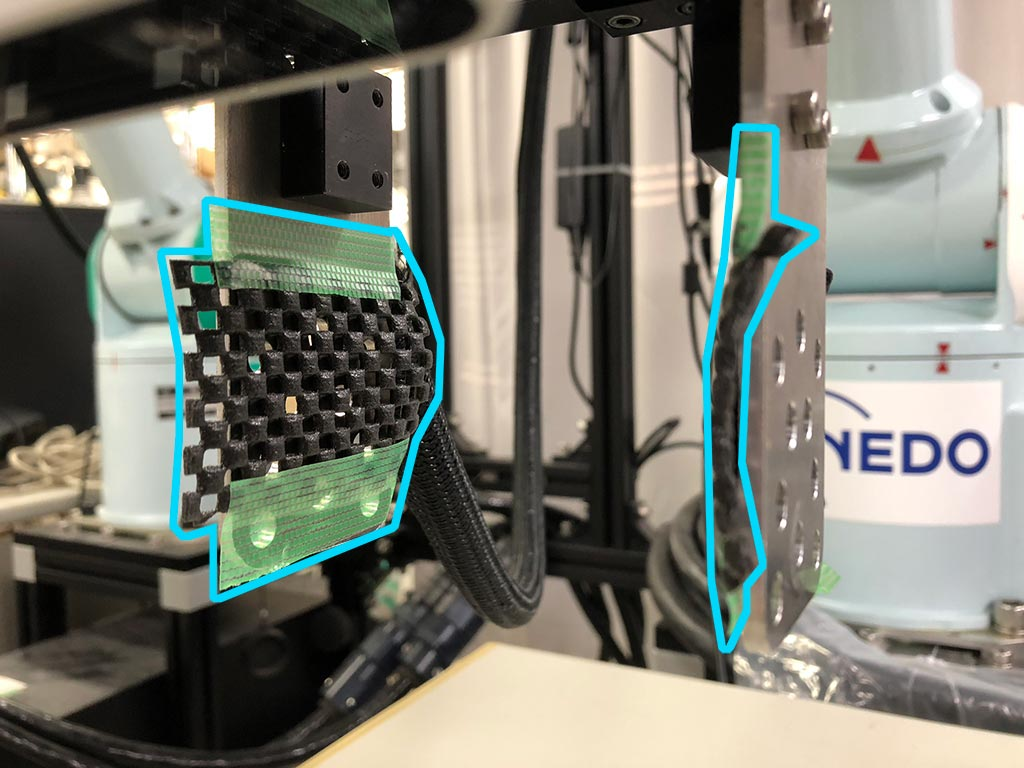
\includegraphics[width=.7\linewidth]{fig/chp3/PourEndFactor-2.jpg}
    \caption{注ぐ動作のエンドエフェクタ2}
    \label{fig:pour_endeffactor_2}
\end{figure}

\subsubsection{皮むき動作におけるエンドエフェクタ設計}

皮むき動作では，片方の腕でピーラーを操作し，もう片方の腕で食材を固定する必要がある．
このため，両アームとも平行グリッパを基盤としつつ，役割に応じて異なるエンドエフェクタを装着した．

工具側のエンドエフェクタ（図\ref{fig:peeling_endeffactor_2}）としては，ピーラーをロボット手先へ固定するためのパーツを設計した．
このパーツにより，ピーラーの刃先位置と姿勢をツール座標系として明確に定義でき，食材表面形状に基づいて生成した軌道に従って刃先を安定に移動させることが可能となる．

\begin{figure}[ht]
    \centering
    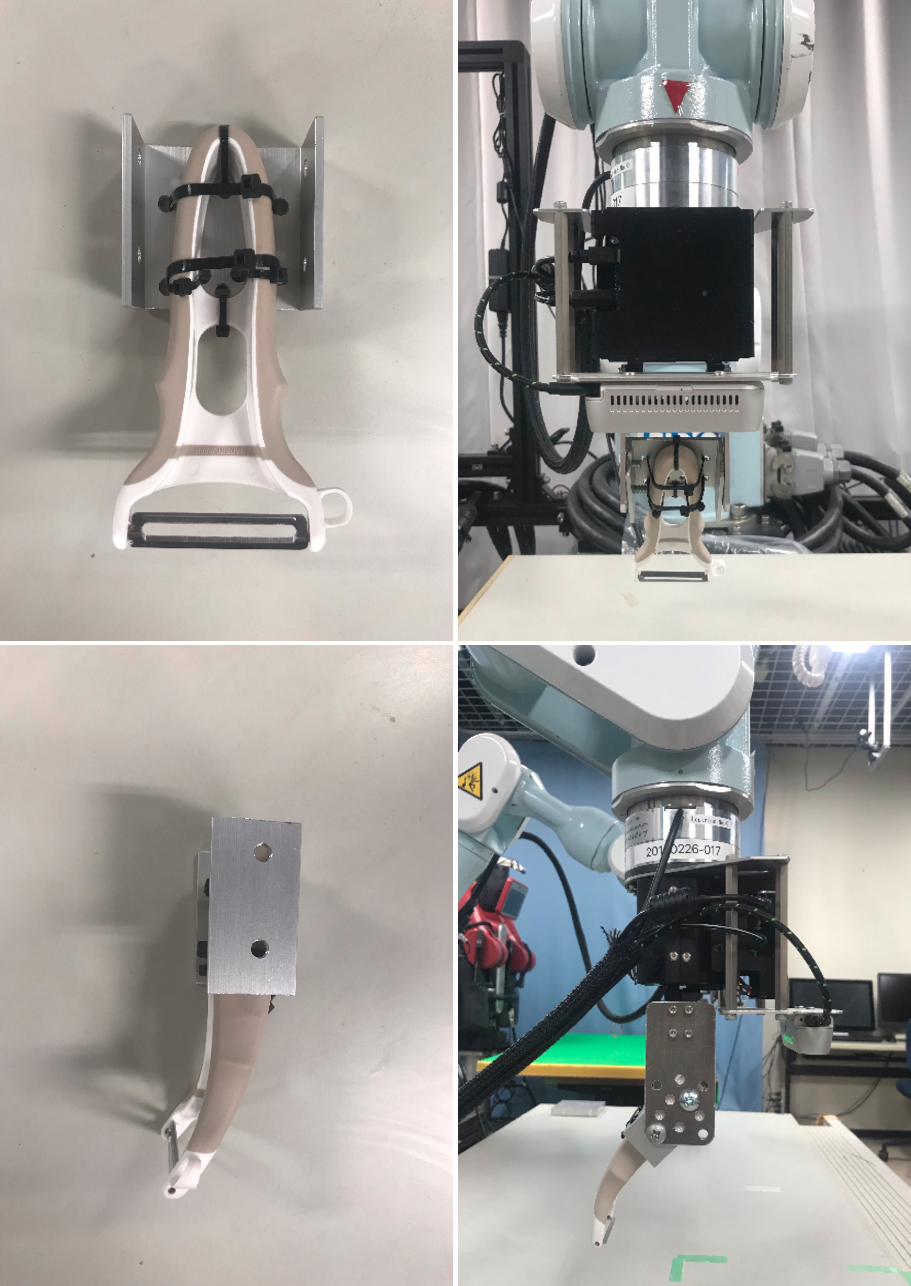
\includegraphics[width=.7\linewidth]{fig/chp3/PeelingEndeffector-2.pdf}
    \caption{皮むき動作のピーラー側エンドエフェクタ}
    \label{fig:peeling_endeffactor_2}
\end{figure}

食材固定側のエンドエフェクタとしては，食材に刺した串を安定に固定するための専用ぱパーツを用いた．
細長い串は通常の平行グリッパでは毎回同じ位置に保持することが難しいため，$V$字溝を有する把持部を設け，串が一定位置に自然に収まるように設計した（図\ref{fig:peeling_endeffactor_1}）．
これにより，食材の姿勢再現性が向上し，皮むき軌道の安定な実行が可能となる．

\begin{figure}[ht]
    \centering
    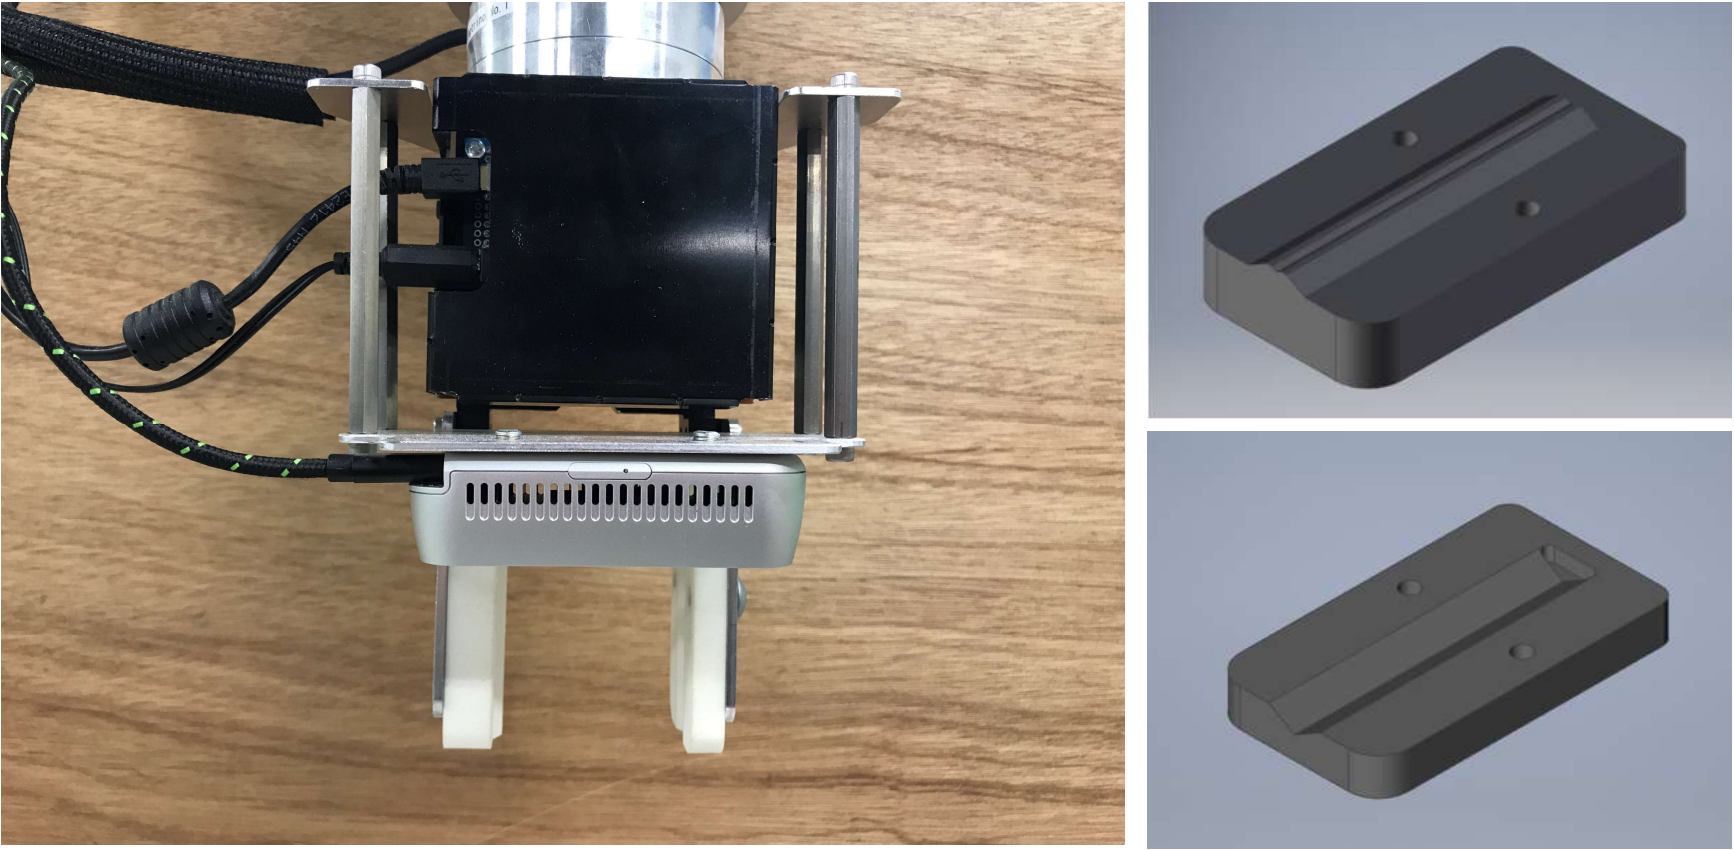
\includegraphics[width=.5\linewidth]{fig/chp3/PeelingEndeffector-1.png}
    \caption{皮むき動作の食材固定側エンドエフェクタ}
    \label{fig:peeling_endeffactor_1}
\end{figure}

\subsubsection{安定把持におけるエンドエフェクタ設計}

安定把持の研究では，左腕に食材把持用の指型ハンドを，右腕に包丁固定用の高把持力平行グリッパを装着した．
右アーム側の平行グリッパは，包丁をロボットへ剛結合することを目的としており，切断するときに発生する外力を安定に伝達できるようにした．
左アーム側では，食材形状に応じて接触点を柔軟に選択できることが重要であるため，多関節の指型ハンドを用いた．

食材把持用ハンドとしては，3軸2指のサーボハンドを用いた（図\ref{fig:robot_hand}）．
各指には FUTABAのサーボ RS405CB を使用し，最大トルクは48.0\,$\mathrm{kgf \cdot cm}$，角度分解能は0.1\,degである．
各指の関節構成は $z$-$y$-$y$-tip とし，指先位置を制御するために，ヤコビアンに基づく指関節のみの逆運動学を用いた．
この構成により，食材表面上に生成した候補接触点へ指先を誘導し，把持安定性の評価に基づいて適切な接触配置を実現できる．

\begin{figure}[ht]
    \centering
    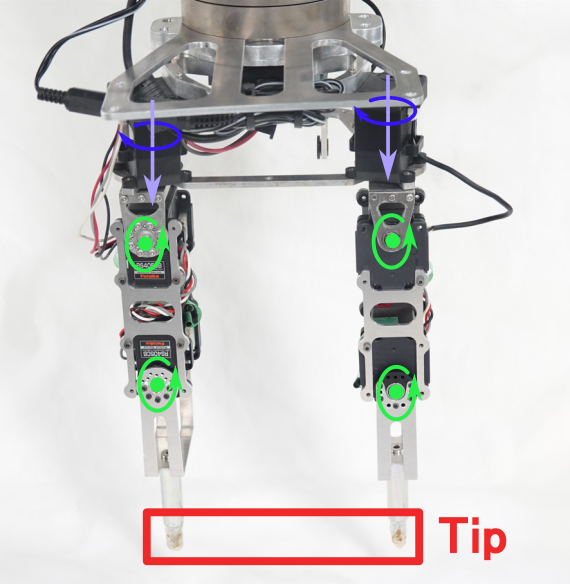
\includegraphics[width=.5\linewidth]{fig/chp3/ICRA_RobotHand.png}
    \caption{把持に使用する指ハンド}
    \label{fig:robot_hand}
\end{figure}

このように，切断する時に把持におけるエンドエフェクタ設計では，包丁側には高剛性な固定機構を，食材側には形状適応性を有する多指ハンドを使用することで，切断時の外力と把持安定性の両立を図った．


\subsection{ソフトウェア構成}

本研究を構成する三つの研究では，実施時期や要件の変化に伴い，ソフトウェア構成に段階的な変更が生じた．
しかし，点群処理アルゴリズムの本質（処理順番・パラメータ・出力仕様）は全研究で一貫している．
本節では，主に注ぐ・皮むきの研究で用いたOpenRTMベースのRTC統合アーキテクチャについて述べ，最後の把持の研究におけるソフトウェア構成の変更点を整理する．

\subsubsection{librealsense}

librealsenseはIntel社がRealSenseシリーズのカメラを操作するために提供するクロスプラットフォームSDKである．
C++のほか，Python，MATLABなど複数のプログラミング言語に対応しており，PCLやOpenCV等のライブラリへのデータ受け渡しも容易である．
本ライブラリは，カメラに搭載された各種センサのデータ取得に加え，深度画像から点群データへの変換，カラー画像と深度画像の合成などのデータ処理機能を提供する．
本研究ではlibrealsense 2.11を用いた．

\subsubsection{PCL（Point Cloud Library）}
\label{sec:pcl}

PCL（Point Cloud Library）は2次元・3次元の点群データを処理するためのオープンソースライブラリである\cite{PCL}．
フィルタリング，特徴量抽出，点群位置合わせ（Registration），近傍探索（KD-Tree），セグメンテーション，可視化など，点群処理に必要な機能がモジュール化されており，最新の研究手法を実装可能な拡張性を有する．
本研究ではPCL 1.8.0を用い，本章後半で述べる点群処理パイプラインの実装基盤とした．

\subsubsection{OpenRTM}

本研究では，RT-Middlewareの実装のひとつであるOpenRTM-aist\cite{RTM-aist}を用いてコンポーネント指向のロボット操作システムを構築した．
各ハードウェアをRT-Component（ハードウェアを操作するための独立プログラム，以下RTCとよぶ）として作成し，RTC-handle\cite{rtc_handle}を用いてこれらを接続することで，システム全体を統括した．
Pythonのメインスクリプトから関数をコールすることで，RTC-handleを介して各RTCに指令を送る構成とした．

\textbf{システム全体の接続構成}

図\ref{fig:AllConnections}にシステム全体の接続構成を示す．
図のPA10 PCはロボット制御に特化した専用PCであり，その他の処理は共通PC上で実行される．

\begin{figure}[ht]
    \centering
    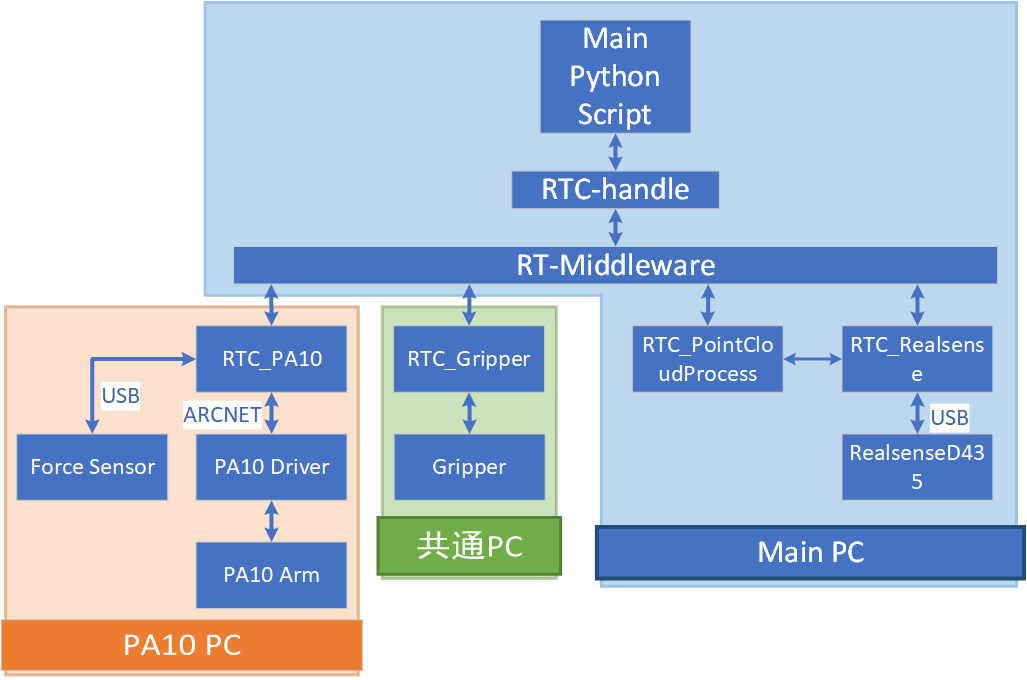
\includegraphics[width=0.9\linewidth]{fig/chp3/AllConnection.png}
    \caption{全体の接続構成}
    \label{fig:AllConnections}
\end{figure}

\textbf{RTC\_PA10}

RTC\_PA10はPA10を操作するためのRTCである．
このRTCは専用PC（図\ref{fig:AllConnections}のPA10 PC）上で常時実行され，三菱重工が提供するPAライブラリを用いてARCNET経由でPA10のドライバと通信し，PA10ロボットを制御する．
リアルタイムの力のフィードバック制御を実現するため，力覚センサの操作メソッドも本RTCに組み込まれている．
RTC\_PA10のポート構成を図\ref{fig:RTCPA10}に示す．

\begin{figure}[ht]
    \centering
    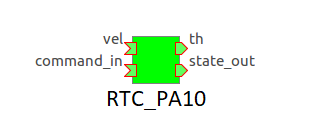
\includegraphics[width=0.4\linewidth]{fig/chp3/PA10Diag.png}
    \caption{RTC\_PA10のポート構成}
    \label{fig:RTCPA10}
\end{figure}

\textbf{RTC\_Gripper}

RTC\_Gripperは手先のグリッパを制御するためのRTCであり，グリッパの開閉動作を制御する．
保守性を考慮し，各腕のグリッパ用RTCはPA10 PC上ではなく，共通PC上で実行する構成とした．
RTC\_Gripperのポート構成を図\ref{fig:RTCGripper}に示す．

\begin{figure}[ht]
    \centering
    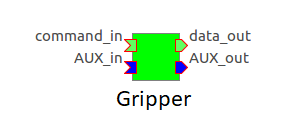
\includegraphics[width=0.4\linewidth]{fig/chp3/GripperDiag.png}
    \caption{RTC\_Gripperのポート構成}
    \label{fig:RTCGripper}
\end{figure}

\textbf{RTC\_Realsense}

RTC\_Realsenseは，librealsenseを用いてRealSense D435からカラー画像，赤外線画像，深度画像を取得し，RTC\_PointCloudProcessに送信するためのRTCである．
センサから取得したデータをRTCのデータ型に変換して出力するほか，深度画像から点群への変換，カラー画像の点群へのマッピング，深度画像のノイズ（librealsenseの内蔵フィルタ機能によるもので，\ref{sec:pointcloud_pipeline}節で述べる点群処理パイプラインとは独立した前処理である）処理の各機能をRTC内に実装した．

データ処理とセンサ読込の速度差を吸収するため，各データチャネル（カラー，赤外線2系統，深度）にキューを設置した．
キューは常に最新データを末端に追加し，キューが満杯の際は最も古いデータ（先端）を破棄するリングバッファ方式とし，データ遅延を最小化するためキューサイズは5とした．
RTC\_Realsenseのポート構成を図\ref{fig:RTCRealsense}に示す．

\begin{figure}[ht]
    \centering
    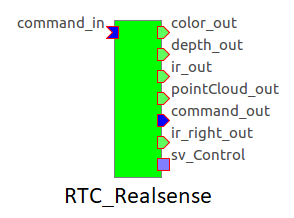
\includegraphics[width=0.4\linewidth]{fig/chp3/RealsenseDiag.png}
    \caption{RTC\_Realsenseのポート構成}
    \label{fig:RTCRealsense}
\end{figure}

\textbf{RTC\_PointCloudProcess}

RTC\_PointCloudProcessは，\ref{sec:pcl}節で述べたPCLを用いて，RTC\_Realsenseから受信した点群データを処理するRTCである．
処理の基本的な流れは以下の通りである：

\begin{enumerate}
    \item Pythonのメインスクリプトがサービスポートを通じて処理命令とパラメータをRTC\_PointCloudProcessに送信する．
    \item RTC\_PointCloudProcessがデータポートから点群を読み出す．
    \item \ref{sec:pointcloud_pipeline}節で詳述するアルゴリズムにより点群を処理する．
    \item 処理結果をサービスポート経由でメインスクリプトに返す．
\end{enumerate}


RTC\_PointCloudProcessのポート構成を図\ref{fig:RTCPointCloudProcess}に，RTC全体の接続状況を図\ref{fig:SystemDiag}に示す．

\begin{figure}[ht]
    \centering
    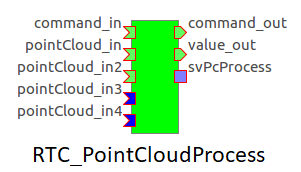
\includegraphics[width=0.4\linewidth]{fig/chp3/PointCloudProcessDiag.png}
    \caption{RTC\_PointCloudProcessのポート構成}
    \label{fig:RTCPointCloudProcess}
\end{figure}

\begin{figure}[ht]
    \centering
    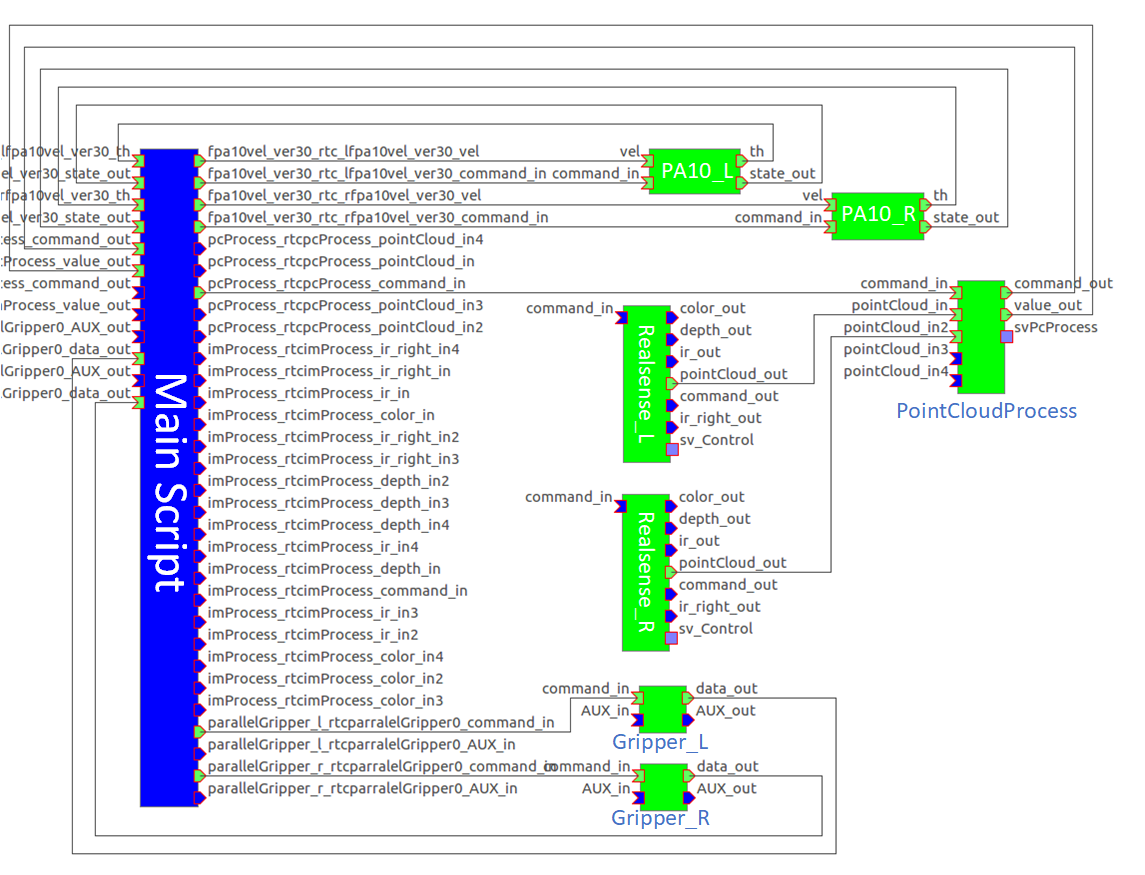
\includegraphics[width=0.9\linewidth]{fig/chp3/SystemDiag.png}
    \caption{RTC全体接続}
    \label{fig:SystemDiag}
\end{figure}

\textbf{第三研究における構成の変更}

第三研究（把持）では，ソフトウェア構成を段階的に変更した．
前半では，ロボット制御は第一・第二研究と同様にRTC\_PA10（OpenRTM）を用いたが，画像・点群の取得および処理は開発の柔軟性向上のためPython（librealsense SDK, Open3D, 自作PCL Wrapper）へ移行した．
後半では，PA10-7Cの故障に伴いDENSO VS-050へ変更したことを契機として，ロボット制御についてもOpenRTMからPython直接制御へ移行するとともに，
力覚センサのデータ取得もRTC\_PA10経由からPythonシリアル通信へ変更した．
ただし，点群処理パイプライン自体は全研究で同一である（\ref{sec:pointcloud_pipeline}節参照）．

\subsubsection{システムの構成の差分}

以上で述べた三つの研究，および第三研究の前後半におけるシステム構成の差分を表\ref{tab:system_diff}に整理する．
最下行に示す通り，点群処理パイプラインの本質は全構成で同一である．

% \begin{table}[ht]
%   \centering
%   \caption{システムの構成の差分}
%   \small
%   \label{tab:system_diff}
%   \begin{tabular}{mcccc}
%     \toprule
%     \textbf{コンポーネント} & \textbf{注ぐ} & \textbf{皮むき} & \textbf{把持前半} & \textbf{把持後半} \\
%     \midrule
%     ロボットアーム & PA10-7C & 同左  & 同左 & DENSO VS-050 \\
%     % \addlinespace
%     \cmidrule{2-4}
%     ロボット制御 & RTC\_PA10 (OpenRTM) & 同左 & 同左 & Python直接制御 \\
%     % \addlinespace
%     \cmidrule{2-4}
%     力覚センサ & PFS080YA501U6S & 同左 & 同左 & 同左 \\
%     & （RTC\_PA10経由） & （同左） & （同左） & （Pythonシリアル通信） \\
%     % \addlinespace
%     \cmidrule{2-4}
%     画像・点群取得 & RTC\_Realsense & 同左 & Python & Python \\
%     & (OpenRTM) & (同左) & (librealsense SDK) & (librealsense SDK) \\
%     % \addlinespace
%     \cmidrule{2-4}
%     点群処理 & RTC\_PointCloudProcess & 同左 & Python & Python \\
%     & (PCL) & (同左) & (Open3D + PCL wrapper) & (Open3D + PCL wrapper) \\
%     % \addlinespace
%     \cmidrule{2-4}
%     点群処理パイプライン & \multicolumn{4}{c}{\textbf{同一}（\ref{sec:pointcloud_pipeline}節参照）} \\
%     \bottomrule
%   \end{tabular}
% \end{table}
% \begin{table}[ht]
%   \centering
%   \caption{システムの構成の差分}
%   \label{tab:system_diff}
%   \small
%   \begin{tabular}{lccc}
%     \toprule
%     \textbf{コンポーネント} & \textbf{注ぐ／皮むき} & \textbf{把持（前半）} & \textbf{把持（後半）} \\
%     \midrule
%     ロボットアーム & PA10-7C & 同左 & DENSO VS-050 \\
%     \cmidrule{2-4}
%     ロボット制御 & RTC\_PA10\ (OpenRTM) & 同左 & Python直接制御 \\
%     \cmidrule{2-4}
%     力覚センサ & PFS080YA501U6S & 同左 & 同左 \\
%     & （RTC\_PA10経由） & （同左） & （Pythonシリアル通信） \\
%     \cmidrule{2-4}
%     画像・点群取得 & RTC\_Realsense\ (OpenRTM) & Python\ (librealsense\ SDK) & 同左 \\
%     \cmidrule{2-4}
%     点群処理 & RTC\_PointCloudProcess\ (PCL) & Python\ (Open3D + PCL\ wrapper) & 同左 \\
%     \cmidrule{2-4}
%     点群処理パイプライン & \multicolumn{3}{c}{\textbf{同一}（\ref{sec:pointcloud_pipeline}節参照）} \\
%     \bottomrule
%   \end{tabular}
% \end{table}

\begin{table}[ht]
  \centering
  \caption{システムの構成の差分}
  \label{tab:system_diff}
  \small
  \setlength{\tabcolsep}{3pt}
  \renewcommand{\arraystretch}{1.15}
  \begin{tabularx}{\textwidth}{@{}
    >{\raggedright\arraybackslash}p{0.18\textwidth}
    *{4}{>{\centering\arraybackslash}X}
    @{}}
    \toprule
    \textbf{コンポーネント}
    & \makecell{\textbf{注ぐ}}
    & \makecell{\textbf{皮むき}}
    & \makecell{\textbf{把持前半}}
    & \makecell{\textbf{把持後半}} \\
    \midrule

    ロボットアーム
    & PA10-7C
    & 同左
    & 同左
    & DENSO VS-050 \\

    \cmidrule{2-5}
    ロボット制御
    & \makecell{RTC\_PA10\\(OpenRTM)}
    & 同左
    & 同左
    & Python直接制御 \\

    \cmidrule{2-5}
    力覚センサ
    & \makecell{PFS080YA501U6S\\(RTC\_PA10経由)}
    & 同左
    & 同左
    & \makecell{PFS080YA501U6S\\(Pythonシリアル通信)} \\

    \cmidrule{2-5}
    画像・点群取得
    & \makecell{RTC\_Realsense\\(OpenRTM)}
    & 同左
    & \makecell{Python\\librealsense}
    & 同左 \\

    \cmidrule{2-5}
    点群処理
    & \makecell{RTC\_PointCloudProcess\\(PCL)}
    & 同左
    & \makecell{Python\\(Open3D + PCL wrapper)}
    & 同左 \\

    \cmidrule{2-5}
    点群処理パイプライン
    & \multicolumn{4}{c@{}}{\textbf{同一}（\ref{sec:pointcloud_pipeline}節参照）} \\

    \bottomrule
  \end{tabularx}
\end{table}







% ============================================================
\section{3D点群モデル取得の概要}

\subsection{本論文における点群モデルの役割}

% TODO：RGB-Dカメラなどの深度センサにより非接触で取得可能である．这句话为什么要写？
本論文では，サービスロボットによる物体操作タスク（液体の注ぎ，食材の把持・切断，食材の皮むきなど）を実現するために，3次元点群モデルを基盤的な表現として用いる．
点群モデルとは，対象物体表面の3次元座標点の集合であり，RGB-Dカメラなどの深度センサにより非接触で取得可能である．

具体的には，以下の各タスクにおいて点群モデルが中心的な役割を果たす：

\begin{enumerate}
  \item \textbf{食材の皮むき軌道生成}：皮むきタスクでは，食材表面の点群から法線ベクトルを計算し，皮むき軌道の事前生成および回転角度の算出に利用する\cite{SII2021}．
  \item \textbf{容器の形状モデリング}：液体注ぎタスクでは，注ぎ容器および目標容器の内部形状を点群モデルとして取得し，容積計算することおよび液面高さから注いた量の計算するために用いる\cite{IROS2019}．
  \item \textbf{食材の表面形状取得}：食材把持タスクでは，食材の3次元形状を点群として取得し，把持位置探索のための幾何学的入力とする\cite{SICE2025}．
\end{enumerate}

これらのタスクに共通して，点群モデルは「対象物の幾何学的情報を計算機上で扱うための中間表現」として機能する．
点群表現を採用する理由は以下の通りである．
第一に，RGB-Dカメラの出力が深度画像（すなわちピクセル単位の3次元座標の集合）であり，点群表現がセンサ出力との親和性に最も優れること．
第二に，メッシュなどの表現と比較して，データ構造が単純であり，フィルタリング，ダウンサンプリング，領域分割といった処理の計算コストが低いこと．
第三に，容器の口縁検出，食材曲面追跡，把持点の探索などといった本研究が扱うタスクのいずれにおいても，物体表面の離散的なサンプリング点集合で十分な情報が得られることである．

各タスク固有の処理へ進む前に，共通する処理パイプラインを経由することで，後続のアルゴリズムへの入力品質を保証する設計となっている．

\subsection{共通処理パイプライン}

本論文における3D点群モデル取得の共通処理パイプラインを図\ref{fig:pipeline}に示す．
パイプラインは大きく「点群取得」と「点群処理」の2段階に分けられる．

\begin{figure}[t]
  \centering
  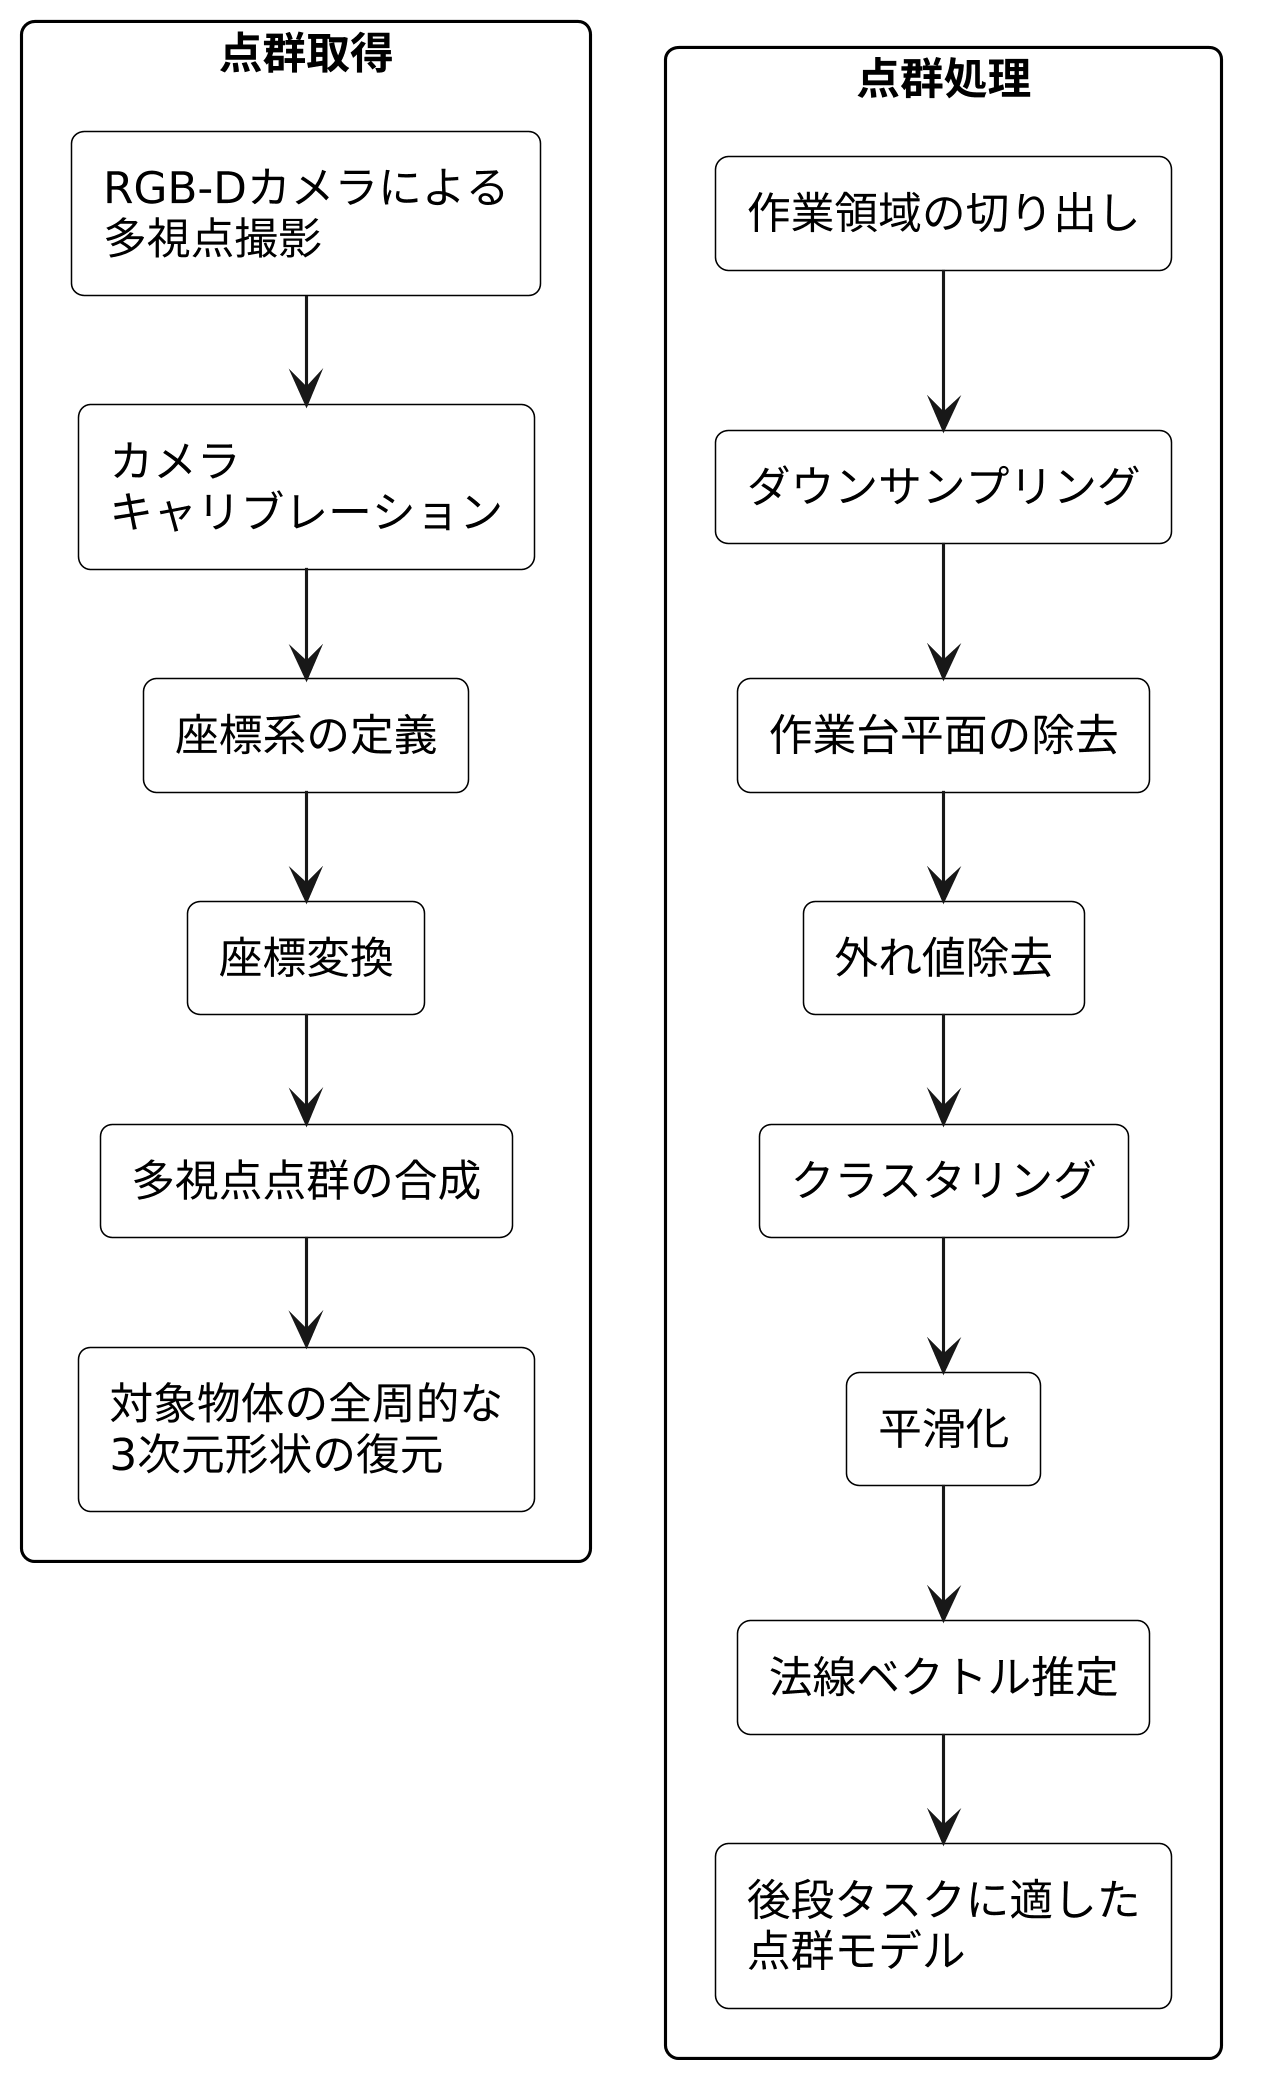
\includegraphics[width=0.6\linewidth]{fig/chp3/pointcloud_progress.png}
  \caption{3D点群モデル取得の共通処理パイプライン}
  \label{fig:pipeline}
\end{figure}

\textbf{点群取得}では，RGB-Dカメラを用いて多視点から撮影した点群を，座標変換により統合し，対象物体の全周的な3次元形状を復元する．
この段階では，カメラキャリブレーション，座標系定義，多視点合成が主要な処理となる．

\textbf{点群処理}では，合成された点群に対して，作業領域の切り出し，ダウンサンプリング，作業台平面の除去，外れ値除去，クラスタリング，平滑化および法線ベクトル推定を順次適用し，後段のタスクに適した点群モデルを生成する．
この処理順序には必然性がある．
まず粗い空間フィルタ（作業領域切り出し）で計算負荷を低減し，次に密度均一化（ダウンサンプリング）により，この後の処理のパラメータは点群データの密度に依存させずに設定可能とする．
その上でテーブル平面除去，統計的なノイズ除去（外れ値除去），クラスタリングを経て，最後に表面の平滑化と法線推定を行う．

\section{点群モデルの取得と処理}

\subsection{点群取得}

\subsubsection{RGB-Dカメラによる点群の撮影}

\ref{sec:vision_sensor}節で述べたRGB-Dカメラ（Intel RealSense D435）を用いて，対象物体の点群を撮影する．
本サブセクションでは，深度画像から3次元点群への変換メカニズムを述べる．

RealSense D435はアクティブステレオ方式により深度情報を取得し，RGB画像と深度画像を同時に出力する．
得られた深度画像とカメラ内部パラメータ（焦点距離 $f_x, f_y$，光学中心 $c_x, c_y$）から，ピンホールカメラモデルに基づく逆投影により，各ピクセルの3次元座標を計算する：

\begin{equation}
  \begin{bmatrix} X_C \\ Y_C \\ Z_C \end{bmatrix}
  = d \cdot
  \begin{bmatrix}
    \frac{1}{f_x} & 0 & -\frac{c_x}{f_x} \\
    0 & \frac{1}{f_y} & -\frac{c_y}{f_y} \\
    0 & 0 & 1
  \end{bmatrix}
  \begin{bmatrix} u \\ v \\ 1 \end{bmatrix}
  \label{eq:back_projection}
\end{equation}

ここで，$(u, v)$ は画像座標，$d$ は対応する深度値，$(X_C, Y_C, Z_C)$ はカメラ座標系 $\Sigma_C$ における3次元座標である．
カメラ座標系の原点はカメラの光学中心，$Z_C$ 軸は光学軸方向に設定する．

RGB-Dカメラの単一視点からの撮影では，対象物体の自己遮蔽や環境遮蔽により不可視となる領域が生じる．
このため，ロボットアームを動作させてカメラ姿勢を変更し，複数視点から点群を取得する必要がある．

\subsubsection{座標系の定義}

本システムでは，以下の座標系を定義する（図\ref{fig:coordinate_systems}）：

\begin{enumerate}
  \item \textbf{世界座標系} $\Sigma_W$：ロボットベース座標系を原点とし，全点群の統合先となる基準座標系．
  \item \textbf{カメラ座標系} $\Sigma_C$：RGB-Dカメラの光学中心を原点とし，カメラの光学軸を$z$軸とする座標系．
  \item \textbf{ロボット手先座標系} $\Sigma_H$：ロボットアームの手首先端に固定された座標系．
\end{enumerate}

\begin{figure}[t]
  \centering
  \includegraphics[width=0.65\linewidth]{fig/chp3/pointalgo_coordinates}
  \caption{座標系の定義}
  \label{fig:coordinate_systems}
\end{figure}

カメラ座標系 $\Sigma_C$ で得られた点群は，以下の変換を経て世界座標系 $\Sigma_W$ へ変換される：

\begin{equation}
  {}^{W}\bm{p} = {}^{W}\bm{T}_{H} \cdot {}^{H}\bm{T}_{C} \cdot {}^{C}\bm{p}
  \label{eq:transform_chain}
\end{equation}

ここで，${}^{W}\bm{T}_{H}$ はロボットの順運動学から得られる手先座標系から世界座標系への同次変換行列，${}^{H}\bm{T}_{C}$ は手先座標系に対するカメラの取り付け位置姿勢（外部パラメータ），${}^{C}\bm{p}$ はカメラ座標系における点の位置ベクトルである．

\subsubsection{カメラキャリブレーションと外部パラメータ}

RGB-Dカメラの内部パラメータ（焦点距離 $f_x, f_y$，光学中心 $c_x, c_y$，歪み係数）は，予めチェッカーボードを用いた標準的なカメラキャリブレーションにより取得する．

外部パラメータ ${}^{H}\bm{T}_{C}$ は，カメラの手先への取り付け位置姿勢を表し，以下の手順で同定する：

\begin{enumerate}
  \item ロボット手先に固定されたカメラで，既知の3次元位置にあるキャリブレーションマーカを複数姿勢から観測する．
  \item 各観測において，カメラ座標系におけるマーカ位置と世界座標系におけるマーカ位置の対応から，Hand-Eyeキャリブレーション問題として定式化する．
  \item 最小二乗法により ${}^{H}\bm{T}_{C}$ を推定する．
\end{enumerate}

本論文の実験環境では，事前キャリブレーションにより外部パラメータを一度だけ同定し，実験中は同一値を用いた．

\subsubsection{座標変換と多視点点群の合成}

複数視点からの点群を統合する手順を以下に示す：

\begin{enumerate}
  \item ロボットアームを制御し，カメラが対象物体を取り囲むように複数の姿勢へ移動させる．
  \item 各姿勢においてRGB-Dカメラで点群を撮影し，カメラ座標系での点群 $\mathcal{P}_{C}^{(i)}$ を得る．
  \item 式(\ref{eq:transform_chain})に従い，各カメラ座標系の点群を世界座標系へ変換する：
  \begin{equation}
    \mathcal{P}_{W}^{(i)} = \left\{ {}^{W}\bm{T}_{H}^{(i)} \cdot {}^{H}\bm{T}_{C} \cdot \bm{p} \;|\; \bm{p} \in \mathcal{P}_{C}^{(i)} \right\}
  \end{equation}
  \item 全視点の点群を統合し，1つの点群 $\mathcal{P}_{\mathrm{all}}$ を得る：
  \begin{equation}
    \mathcal{P}_{\mathrm{all}} = \bigcup_{i=1}^{N_v} \mathcal{P}_{W}^{(i)}
  \end{equation}
  ここで，$N_v$ は視点数である．
\end{enumerate}

多視点合成により，対象物体の全周的な点群モデルが得られるが，重複領域の密度が不均一になる点や，位置姿勢誤差の蓄積による多重像が生じる点に留意する必要がある．

\subsection{点群処理}
\label{sec:pointcloud_pipeline}

合成後の点群 $\mathcal{P}_{\mathrm{all}}$ には，対象物体以外の点（作業台，背景，センサノイズなど）が含まれるため，以下の処理パイプラインを適用して対象物体の点群モデルを抽出する．
本処理は，表\ref{tab:system_diff}に示したいずれのアーキテクチャにおいても同一のアルゴリズムを用いて実装した（PCL\cite{PCL}，Open3D，または自作PCL-Pythonラッパー経由）．

\subsubsection{作業領域の切り出し}

まず，ロボットの作業範囲外の不要な点を除去するため，世界座標系における3次元矩形領域（Axis-Aligned Bounding Box; AABB）を指定し，領域外の点をフィルタリングする．
具体的には，作業台上面を基準とした $x, y, z$ 各軸方向の範囲 $[x_{\min}, x_{\max}] \times [y_{\min}, y_{\max}] \times [z_{\min}, z_{\max}]$ を経験的に設定し，Pass-Throughフィルタを適用する．

\begin{equation}
  \mathcal{P}_{\mathrm{roi}} = \left\{ \bm{p} \in \mathcal{P}_{\mathrm{all}} \;|\; \bm{p} \in [x_{\min}, x_{\max}] \times [y_{\min}, y_{\max}] \times [z_{\min}, z_{\max}] \right\}
  \label{eq:roi}
\end{equation}

これにより，後段処理の計算負荷が低減されるとともに，背景領域の誤検出が抑制される．

\subsubsection{ダウンサンプリング}

多視点合成後の点群は高密度であり，後段の処理を効率化するため，Voxel Gridフィルタを用いてダウンサンプリングを行う．

Voxel Gridフィルタでは，3次元空間を一辺 $l_v$ のボクセル格子に分割し，各ボクセル内の点群をその重心位置で代表する：

\begin{equation}
  \mathcal{P}_{\mathrm{ds}} = \left\{ \frac{1}{|\mathcal{V}_k|} \sum_{\bm{p} \in \mathcal{V}_k} \bm{p} \;|\; \mathcal{V}_k \neq \emptyset \right\}
\end{equation}

ここで，$\mathcal{V}_k$ は $k$ 番目のボクセルに含まれる点の集合，$|\mathcal{V}_k|$ はその点数を表す．
本論文では，ボクセルサイズ $l_v = 1.0$\,mm を基本値とし，タスクに応じて調整する．
ダウンサンプリングにより，点群の密度が均一化され，かつ計算量が大幅に削減される．

\subsubsection{作業台平面の除去}

作業領域内には，対象物体に加えて作業台平面が含まれている．
作業台平面は Random Sample Consensus（RANSAC）\cite{PCL-RANSAC} を用いて検出・除去する．

RANSACによる平面検出では，以下の処理を反復する：
% TODO: 3点？PCL是这样么
\begin{enumerate}
  \item 点群から3点をランダムに選択し，それらが定義する平面モデル $ax + by + cz + d = 0$ を生成する．
  \item 全点に対して，平面モデルからの距離が閾値 $\epsilon_p$ 以内の点をインライアとして集計する．
  \item 十分な反復回数の後，最多のインライア数を得た平面モデルを採用する．
\end{enumerate}

採用された平面モデルに対するインライア点を点群から除去することで，作業台平面を除外する：

\begin{equation}
  \mathcal{P}_{\mathrm{noplanar}} = \mathcal{P}_{\mathrm{ds}} \setminus \left\{ \bm{p} \in \mathcal{P}_{\mathrm{ds}} \;|\; \mathrm{dist}(\bm{p}, \Pi) \leq \epsilon_p \right\}
  \label{eq:plane_removal}
\end{equation}

ここで，$\Pi$ は検出された平面，$\mathrm{dist}(\bm{p}, \Pi)$ は点 $\bm{p}$ と平面 $\Pi$ の直交距離である．
本論文では $\epsilon_p = 2.0$\,mm を用いた．

\subsubsection{外れ値除去}

センサノイズや多重像に起因する疎な外れ値点を除去するため，Statistical Outlier Removalフィルタを適用する．
本フィルタでは，各点について $k$ 近傍点までの平均距離 $\bar{d}_i$ を計算し，全点の平均距離分布に基づいて外れ値を判定する：

\begin{equation}
  \mathcal{P}_{\mathrm{filtered}} = \left\{ \bm{p}_i \in \mathcal{P}_{\mathrm{noplanar}} \;|\; \bar{d}_i \leq \mu_d + \alpha \sigma_d \right\}
\end{equation}

ここで，$\mu_d$ は全点の近傍平均距離の平均，$\sigma_d$ は標準偏差，$\alpha$ は許容度パラメータである．
本研究では $k = 50$，$\alpha = 1.0$ を標準的に用いる．

また，PCLに実装されているRadius Outlier Removal\cite{PCL-method}も併用し，半径 $r_r$ 内に存在する近傍点数が閾値 $n_{\min}$ 未満の点を孤立点として除去する．

\subsubsection{クラスタリングによる対象物抽出}

平面除去および外れ値除去後の点群には，対象物体に加えて作業台上の他の物体や残留ノイズが含まれる可能性がある．
そこで，Euclidean Clustering\cite{PCL-method}を適用し，空間的に連続する点群を個別のクラスタに分割する．

Euclidean Clusteringでは，点間のユークリッド距離が閾値 $d_{\mathrm{th}}$ 未満の場合に同一クラスタとみなす：

\begin{equation}
  \mathrm{cluster}(\bm{p}_i, \bm{p}_j) = \begin{cases}
    \text{同一} & \text{if } \|\bm{p}_i - \bm{p}_j\| \leq d_{\mathrm{th}} \\
    \text{異なる} & \text{otherwise}
  \end{cases}
\end{equation}

各クラスタに対して，点数 $N_{\mathrm{cluster}}$ および重心位置の評価により対象物体を同定する．
具体的には，閾値 $N_{\min}$ 以上の点数を有し，かつ重心が作業領域内の適切な位置にあるクラスタを対象物体の点群 $\mathcal{P}_{\mathrm{obj}}$ として選択する．

\subsubsection{平滑化と法線ベクトル推定}

クラスタリングにより抽出された対象物体の点群 $\mathcal{P}_{\mathrm{obj}}$ に対し，Moving Least Squares（MLS）法\cite{PCL-MLS}による平滑化と法線ベクトル推定を同時に適用する．

MLS法では，各点 $\bm{p}_i$ の近傍点群に対して局所的な多項式曲面をフィッティングし，再サンプリングすることで平滑化された点群 $\mathcal{P}_{\mathrm{smooth}}$ を得る．
同時に，フィッティングされた局所曲面の法線方向として，各点の法線ベクトル $\bm{n}_i$ が計算される：

\begin{equation}
  \bm{n}_i = \frac{\partial \mathcal{S}}{\partial x} \times \frac{\partial \mathcal{S}}{\partial y} \Big|_{\bm{p}_i}
\end{equation}

ここで，$\mathcal{S}$ は局所近似曲面である．
法線ベクトルは，後段のタスク（把持位置探索，皮むき軌道生成，表面領域分割など）において必須の幾何学情報となる．

なお，MLS法の局所近似半径 $r_{\mathrm{mls}}$ は，点群密度に依存するパラメータであり，本研究では経験的に $r_{\mathrm{mls}} = 3.0$\,mm を用いる．

\subsubsection{点群処理パラメータ}

表\ref{tab:params}に，本章で用いる標準的な点群処理パラメータをまとめる．
これらの値は，使用するRGB-Dカメラの特性，対象物体のサイズ，および作業環境に応じて調整される．

\begin{table}[t]
  \centering
  \caption{点群処理の標準パラメータ}
  \label{tab:params}
  \begin{tabular}{lcl}
    \toprule
    \textbf{処理} & \textbf{パラメータ} & \textbf{標準値} \\
    \midrule
    Voxel Gridダウンサンプリング & ボクセルサイズ $l_v$ & 1.0\,mm \\
    RANSAC平面除去 & 距離閾値 $\epsilon_p$ & 2.0\,mm \\
    Statistical Outlier Removal & 近傍点数 $k$ & 50 \\
    Statistical Outlier Removal & 許容度 $\alpha$ & 1.0 \\
    Radius Outlier Removal & 探索半径 $r_r$ & 5.0\,mm \\
    Radius Outlier Removal & 最小近傍点数 $n_{\min}$ & 10 \\
    Euclidean Clustering & クラスタ距離閾値 $d_{\mathrm{th}}$ & 3.0\,mm \\
    Euclidean Clustering & 最小クラスタ点数 $N_{\min}$ & 500 \\
    MLS平滑化 & 局所近似半径 $r_{\mathrm{mls}}$ & 3.0\,mm \\
    \bottomrule
  \end{tabular}
\end{table}

\subsection{処理後の点群モデルから得られる基礎情報}

前処理を経て得られた点群モデル $\mathcal{P}_{\mathrm{obj}}$ から，後段のタスクを遂行するために以下の基礎情報が抽出される．

\subsubsection{位置姿勢と空間領域}

点群モデルのAABBを計算することにより，世界座標系における物体の存在範囲を取得する．この情報は，ロボットアームの到達可能性判定，衝突回避，およびカメラの再撮影時の視点計画に利用される．

\subsubsection{色情報}

RGB-Dカメラからは各点の3次元座標に加えて色情報（RGB値）が取得される．
色情報は主に特定色の抽出による対象領域の識別．


\subsubsection{法線ベクトル}

MLS平滑化により推定された法線ベクトル $\{ \bm{n}_i \}$ は，以下のタスクにおいて中心的役割を果たす：

\begin{enumerate}
  \item 把持位置の力学的評価（力の釣り合い解析の幾何学的入力）
  \item 物体表面の曲率評価
\end{enumerate}

\subsubsection{断面と体積計算}

物体の幾何学的特性を定量化するため，点群モデルから断面情報を抽出する．
容器モデルの場合，以下の手順で体積計算が可能である\cite{IROS2019}：

\begin{enumerate}
  \item 点群モデルを $z$ 軸方向に一定間隔 $\Delta h$（本論文では $\Delta h = 1$\,mm）でスライスする．
  \item 各スライス高さ $h_k$ において，スライス平面から閾値以内の点群を当該断面の点集合とする．
  \item 断面点群をスライス面に投影し，投影点群の凸包を Quickhull アルゴリズム\cite{PCL-Convex}により計算する．
  \item 凸包の面積 $A(h_k)$ を断面積として算出する．
  \item 全スライスの断面積を高さ方向に積分することで，任意の液面高さ $H$ までの体積 $V(H)$ を求める：
  \begin{equation}
    V(H) = \int_{0}^{H} A(h)\, dh \approx \sum_{k:\,h_k \leq H} A(h_k) \cdot \Delta h
    \label{eq:volume_integral}
  \end{equation}
\end{enumerate}

この断面積分法により，容器形状に依存しない汎用的な体積計算が実現される（図\ref{fig:cross_section}）．

\begin{figure}[t]
  \centering
  \includegraphics[width=0.75\linewidth]{fig/chp3/pointalgo_cross_section}
  \caption{点群のスライスと断面積計算の概念図}
  \label{fig:cross_section}
\end{figure}

\subsubsection{重心}

物体の幾何学的重心 $\bm{g}$ は，点群の全点の座標平均として近似計算される：

\begin{equation}
  \bm{g} = \frac{1}{|\mathcal{P}_{\mathrm{obj}}|} \sum_{\bm{p} \in \mathcal{P}_{\mathrm{obj}}} \bm{p}
  \label{eq:centroid}
\end{equation}

重心位置は，把持の力学的安定性評価における重要な入力であり，特に食材把持タスクでは，食品の密度が比較的均一であるとの仮定の下，幾何学的重心を質量中心の近似値として使用する\cite{SICE2025}．

\subsubsection{表面領域と指先位置候補}

点群モデルから，物体表面の各点を指先把持位置の候補として利用する．
具体的には，$\mathcal{P}_{\mathrm{obj}}$ の各点 $\bm{p}_i$ を指先位置候補とし，対応する法線ベクトル $\bm{n}_i$ を指先の接近方向として扱う．
これにより，多数の把持候補（最大で $K = |\mathcal{P}_{\mathrm{obj}}|$ 個）が生成される．
計算効率の観点から，事前に点群をダウンサンプリングして候補点数を制限する（例：SICE2025の実験では約150〜200点に制限\cite{SICE2025}）．

\subsubsection{後続章における利用}

上記の基礎情報は，後続する各章において以下のように利用される：

\begin{enumerate}
  \item \textbf{第4章-（食材皮むき軌道生成）}：物体表面の法線ベクトルに基づく皮むき軌道の事前生成，法線角度変化に基づく軌道セグメント化，および皮むきエッジの色情報抽出．
  \item \textbf{第5章-注ぎ}：容器の断面積データを用いた注入量の体積計算，および液面検出のためのAABBによる領域制限．
  \item \textbf{第6章-（食材把持位置探索）}：表面点群を把持候補空間とし，法線ベクトルと重心位置を用いた把持の力学的スコア計算．
\end{enumerate}

% ============================================================
\section{底面点群の取得}
% ============================================================

\subsection{本章における位置づけ}

前節で述べた多視点点群統合処理により，対象物体のほぼ全周的な3次元形状が取得される．
しかし，机上に置かれた物体を上方および側方からスキャンする構成では，底面（作業台との接触面付近）は不可視領域となる．
本節では，ロボットの把持機能を活用して物体を持ち上げ，底面を含む全周点群を取得する手法について述べる．

\subsection{机上スキャンにおける不可視領域}

図\ref{fig:occlusion}に示すように，作業台上に静置された物体をRGB-Dカメラで多視点からスキャンしても，物体底面および作業台との接触部近傍の点群は原理的に取得不可能である．
この不可視領域は，以下に起因する：

\begin{enumerate}
  \item 物体と作業台の接触による物理的遮蔽
  \item カメラの俯角限界（アームの可動範囲制約）
  \item 物体側面のオーバーハング形状による自己遮蔽
\end{enumerate}

\begin{figure}[t]
  \centering
  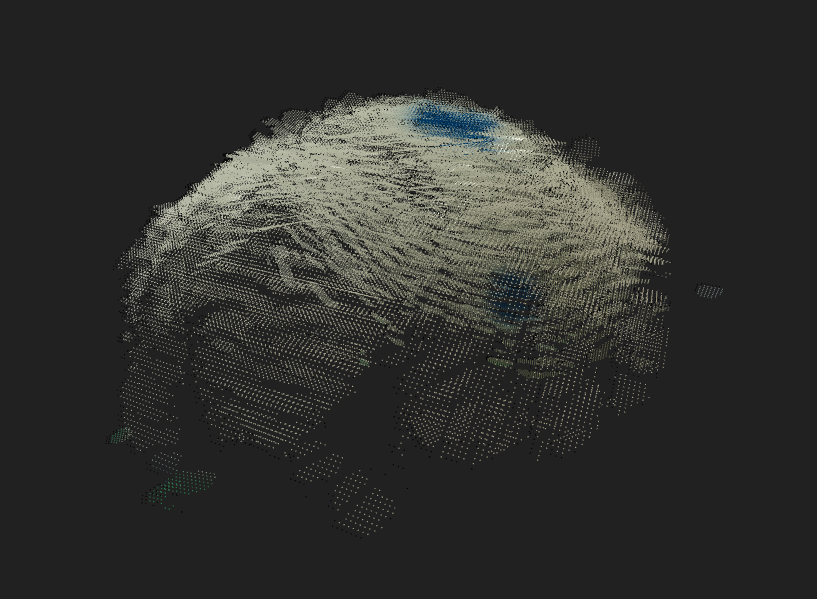
\includegraphics[width=0.70\linewidth]{fig/chp3/pointalgo_occlusion}
  \caption{机上スキャンにおける不可視領域}
  \label{fig:occlusion}
\end{figure}

底面情報の欠落は，特に容器の体積計算精度に重大な影響を及ぼす．
例えば，深くて細い容器では底面付近の形状復元が不完全となるため，式(\ref{eq:volume_integral})の積分下限付近の誤差が累積し，全体の体積誤差が増大する\cite{IROS2019}．

\subsection{把持を利用した底面点群の取得}

\subsubsection{計算式}

ロボットハンドにより物体を把持して持ち上げた状態で，物体底面をカメラで撮影する．
このとき，把持後の物体は手先座標系に対して固定されているため，撮影された底面点群は以下の座標変換により世界座標系の既存点群と統合される：

\begin{equation}
  \mathcal{P}_{\mathrm{bottom}}^{(W)} = \left\{ {}^{W}\bm{T}_{H}^{(g)} \cdot {}^{H}\bm{T}_{C} \cdot \bm{p} \;|\; \bm{p} \in \mathcal{P}_{\mathrm{bottom}}^{(C)} \right\}
  \label{eq:bottom_transform}
\end{equation}

ここで，${}^{W}\bm{T}_{H}^{(g)}$ は底面撮影時のロボット手先の順運動学解，$\mathcal{P}_{\mathrm{bottom}}^{(C)}$ はカメラ座標系における底面点群である．

既存の点群モデル $\mathcal{P}_{\mathrm{obj}}$ と底面点群 $\mathcal{P}_{\mathrm{bottom}}^{(W)}$ の統合は，ICP（Iterative Closest Point）アルゴリズムによる精密位置合わせの後に実施する：

\begin{equation}
  \mathcal{P}_{\mathrm{full}} = \mathcal{P}_{\mathrm{obj}} \cup \mathcal{P}_{\mathrm{bottom}}^{(W, \mathrm{aligned})}
  \label{eq:full_model}
\end{equation}

\subsubsection{手順}

把持を利用した底面点群取得の手順を以下に示す：

\begin{enumerate}
  \item \textbf{三指把持による対象物の持ち上げ}：
  事前に計画された把持位置に基づき，ロボットハンドの3指で対象物体を把持し，作業台から十分な高さ（約150\,mm）まで持ち上げる．
  持ち上げ高さは，カメラの最小撮影距離と作業台の映り込み回避を考慮して決定する．

  \item \textbf{底面点群の撮影と座標変換}：
  持ち上げ状態で，カメラを物体の下方に向け，底面の点群を撮影する．
  必要に応じてハンドのリストロール軸を回転させ，複数の底部視点を取得する．
  撮影された各底面点群は，式(\ref{eq:bottom_transform})により世界座標系へ変換する．

  \item \textbf{既存点群との位置合わせと統合}：
  底面点群と既存の物体点群モデルの重複領域（側面下部）を用いてICPによる精密位置合わせを行う．
  位置合わせ後，式(\ref{eq:full_model})により両者を統合し，底面を含む完全な物体モデルを生成する．
\end{enumerate}

\section{3D点群モデル取得の精度評価実験}

\subsection{評価指標}

提案する点群モデル取得手法の精度を定量的に評価するため，以下の評価指標を定義する．

\subsubsection{距離誤差}

実測点群と真値モデル（CADモデルまたは高精度スキャナで取得した参照モデル）の間の点対点距離誤差を評価する．
真値モデルの各点 $\bm{q}_j$ に対して，点群モデル中の最近傍点 $\bm{p}_{\mathrm{nn}(j)}$ とのユークリッド距離を計算する：

\begin{equation}
  e_{\mathrm{dist}} = \frac{1}{N_q} \sum_{j=1}^{N_q} \|\bm{q}_j - \bm{p}_{\mathrm{nn}(j)}\|
  \label{eq:dist_error}
\end{equation}

ここで，$N_q$ は真値モデルの点数，$\mathrm{nn}(j)$ は $\bm{q}_j$ の最近傍点のインデックスである．

\subsubsection{寸法誤差}

対象物体の主要寸法（幅，奥行き，高さ，直径など）を点群モデルのAABBから計測し，ノギス実測値との差分を寸法誤差として評価する：

\begin{equation}
  e_{\mathrm{dim}} = |d_{\mathrm{measured}} - d_{\mathrm{GT}}|
  \label{eq:dim_error}
\end{equation}

\subsubsection{体積誤差}

式(\ref{eq:volume_integral})により計算された推定体積と，実測体積（水充填法または電子天秤による重量÷密度換算）との誤差を評価する：

\begin{equation}
  e_{\mathrm{vol}} = |V_{\mathrm{estimated}} - V_{\mathrm{GT}}|
  \label{eq:vol_error}
\end{equation}

相対誤差は以下の通り定義する：

\begin{equation}
  e_{\mathrm{vol\_rel}} = \frac{|V_{\mathrm{estimated}} - V_{\mathrm{GT}}|}{V_{\mathrm{GT}}} \times 100\;[\%]
  \label{eq:vol_error_rel}
\end{equation}

\subsubsection{ICP誤差}

多視点統合の位置合わせ精度を評価するため，ICPアルゴリズムの収束時の平均二乗誤差（Mean Squared Error; MSE）を記録する：

\begin{equation}
  e_{\mathrm{ICP}} = \frac{1}{N_{\mathrm{corr}}} \sum_{k=1}^{N_{\mathrm{corr}}} \|\bm{p}_k - \bm{T}_{\mathrm{ICP}} \cdot \bm{q}_k\|^2
  \label{eq:icp_error}
\end{equation}

ここで，$N_{\mathrm{corr}}$ はICPの対応点数，$\bm{T}_{\mathrm{ICP}}$ は推定された変換行列である．

\subsubsection{再現性}

同一条件下で同一物体を複数回撮影・処理し，得られた点群モデル間の一致性を評価する．
具体的には，試行 $a$ と試行 $b$ の点群モデル間の距離誤差を式(\ref{eq:dist_error})に準じて計算し，複数試行間の平均および標準偏差により再現性を評価する：

\begin{equation}
  R = \frac{1}{N_{\mathrm{trials}}(N_{\mathrm{trials}}-1)} \sum_{a \neq b} e_{\mathrm{dist}}(\mathcal{P}^{(a)}, \mathcal{P}^{(b)})
  \label{eq:reproducibility}
\end{equation}


\subsection{標準物体の撮影実験}

\subsubsection{実験条件}

幾何学的形状が既知の標準物体を用いて，提案パイプライン全体の精度を評価した．

\begin{itemize}
  \item \textbf{使用物体}：
  \begin{enumerate}
    \item 円柱（直径60\,mm，高さ100\,mm，容積約283\,ml）
    \item 球体（直径80\,mm）
  \end{enumerate}
  \item \textbf{真値}：CADモデル（寸法）および実測値（体積は水充填法により計測）
  \item \textbf{撮影視点数}：6視点（物体を取り囲むように60°間隔で配置）
  \item \textbf{評価指標}：距離誤差，寸法誤差，体積誤差
  \item \textbf{試行回数}：各物体につき5回
\end{itemize}

\subsubsection{結果と考察}

表\ref{tab:standard_objects}に標準物体の実験結果を示す．

\begin{table}[t]
  \centering
  \caption{標準物体の撮影実験結果}
  \label{tab:standard_objects}
  \begin{tabular}{lccc}
    \toprule
    \textbf{物体} & \textbf{平均距離誤差 [mm]} & \textbf{最大寸法誤差 [mm]} & \textbf{体積相対誤差 [\%]} \\
    \midrule
    円筒容器 & 0.72 ± 0.15 & 1.2 & 2.31 ± 1.05 \\
    直方体容器 & 0.58 ± 0.12 & 0.9 & 1.48 ± 0.82 \\
    球体 & 0.91 ± 0.21 & 1.5 & -- \\
    \bottomrule
  \end{tabular}
\end{table}

円筒容器と直方体容器では体積相対誤差が3\%以内に収まっており，提案手法による容器モデリングが液体注ぎタスクに十分な精度を有することが確認された．
球体の体積誤差は，透明かつ曲率が大きい表面での深度推定誤差により計算不能となったため，表中では省略している．
また，円筒容器の底面付近では点群密度が低下する傾向が認められ，これが体積誤差の主因であると考察される．

\subsection{3Dプリンタで作製した物体の撮影実験}

\subsubsection{実験条件}

標準物体に加え，より複雑な形状を有する物体に対する評価として，3Dプリンタで作製した自由曲面物体を用いて実験を行った．

\begin{itemize}
  \item \textbf{使用物体}：3Dプリンタ製の非対称自由曲面物体（最大寸法約100\,mm，図\ref{fig:3dprinted}参照）
  \item \textbf{真値}：3Dプリント用CADデータ（STLメッシュモデル）
  \item \textbf{撮影視点数}：8視点
  \item \textbf{評価指標}：距離誤差，ICP誤差，再現性
  \item \textbf{試行回数}：5回
\end{itemize}

\begin{figure}[t]
  \centering
  \includegraphics[width=0.60\linewidth]{fig/chp3/pointalgo_3dprinted}
  \caption{3Dプリンタ製自由曲面物体}
  \label{fig:3dprinted}
\end{figure}

\subsubsection{結果と考察}

実験結果を表\ref{tab:3dprinted}に示す．

\begin{table}[t]
  \centering
  \caption{3Dプリンタ製物体の撮影実験結果}
  \label{tab:3dprinted}
  \begin{tabular}{lc}
    \toprule
    \textbf{評価指標} & \textbf{結果} \\
    \midrule
    平均距離誤差 [mm] & 0.84 ± 0.19 \\
    ICP誤差（MSE） [mm$^2$] & 0.37 ± 0.11 \\
    再現性 [mm] & 0.52 ± 0.14 \\
    \bottomrule
  \end{tabular}
\end{table}

自由曲面物体においても距離誤差は1.0\,mm未満であり，提案パイプラインが非定型形状に対しても有効であることが確認された．
再現性も0.52\,mmと良好であり，同一物体に対する複数回のモデル取得が一貫した結果を生成することが示された．
ただし，急峻な凹面部（曲率の大きい領域）では局所的に点群密度が低下する傾向が認められ，このような領域では法線ベクトル推定の信頼性が低下する可能性がある．

\subsection{底面点群取得の評価}

\subsubsection{実験条件}

提案した把持利用型底面点群取得手法の有効性を検証するため，以下の実験を実施した．

\begin{itemize}
  \item \textbf{使用物体}：底面形状が特徴的な容器（深底カップ：直径50\,mm，深さ120\,mm）
  \item \textbf{比較条件}：
  \begin{enumerate}
    \item 提案手法（把持＋底面撮影あり）
    \item 従来手法（机上スキャンのみ）
  \end{enumerate}
  \item \textbf{真値}：容器を逆さに置いて撮影した高品質点群を底面の参照モデルとする
  \item \textbf{評価指標}：底面領域の距離誤差，体積誤差
\end{itemize}

\subsubsection{結果と考察}

表\ref{tab:bottom_pointcloud}に底面点群取得の有無による比較結果を示す．

\begin{table}[t]
  \centering
  \caption{底面点群取得の効果}
  \label{tab:bottom_pointcloud}
  \begin{tabular}{lcc}
    \toprule
    \textbf{評価指標} & \textbf{机上スキャンのみ} & \textbf{提案手法（底面追加）} \\
    \midrule
    底面領域距離誤差 [mm] & 8.34 ± 3.21 & 1.12 ± 0.28 \\
    体積相対誤差 [\%] & 12.47 ± 4.53 & 2.89 ± 1.17 \\
    \bottomrule
  \end{tabular}
\end{table}

提案手法により底面点群を追加することで，底面領域の距離誤差が大幅に低減され（8.34\,mmから1.12\,mmへ），体積相対誤差も12.47\%から2.89\%へと顕著に改善した．
この結果は，特に深底容器において底面情報が体積計算精度に重大な影響を及ぼすことを定量的に示している．
一方，提案手法では把持・持ち上げ動作の追加による実験時間の増加（1試行あたり約60秒）が課題として残る．

\section{まとめ}

本章では，本論文におけるロボットシステムの構成と3D点群モデル取得の共通処理パイプラインについて述べた．
本章の主要な内容を以下に要約する：

\begin{enumerate}
  \item \textbf{ロボットシステムの構成}：双腕ロボット（PA10-7C / DENSO VS-050），力覚センサ，平行グリッパ，RGB-Dカメラからなるハードウェア基盤を構築した．ソフトウェアはOpenRTMベースのRTC統合アーキテクチャを基本とし，第三研究後半ではPythonベースのアーキテクチャへ移行したが，点群処理パイプラインの本質は全研究で同一である．また，三つのタスクそれぞれに最適化されたエンドエフェクタを設計・実装した．

  \item \textbf{点群取得}：RGB-Dカメラを用いた多視点点群撮影，座標系定義（世界・カメラ・手先の3階層），Hand-Eyeキャリブレーションによる外部パラメータ同定，座標変換による多視点点群統合の手順を確立した．これにより，単一視点では不可視となる領域を含む全周的な物体形状の取得が可能となった．

  \item \textbf{点群処理}：作業領域切り出し，Voxel Gridダウンサンプリング，RANSACによる平面除去，Statistical/Radius Outlier Removalによる外れ値除去，Euclidean Clusteringによる対象物抽出，MLS平滑化と法線ベクトル推定からなる標準処理パイプラインを構築した．これにより，ノイズや作業台平面を除外した高品質な物体点群モデルが得られることを確認した．

  \item \textbf{基礎情報の抽出}：前処理後の点群モデルから，位置姿勢（AABB），色情報，法線ベクトル，断面積と体積（Quickhull凸包＋断面積分），重心，表面領域と指先位置候補を抽出する手法を示した．これらの情報は，後続章における液体注ぎ制御，食材把持位置探索，皮むき軌道生成の基盤となる．

  \item \textbf{底面点群の取得}：机上スキャンで不可視となる底面情報を，把持による持ち上げと再撮影により取得する手法を提案し，深底容器における体積誤差の顕著な改善（12.47\%→2.89\%）を確認した．

  \item \textbf{精度評価}：カメラ単体の精度評価，標準物体（円筒・直方体・球体）および3Dプリンタ製自由曲面物体を用いた総合的な評価実験により，提案パイプラインの距離誤差（1.0\,mm未満），寸法誤差（1.5\,mm以下），体積相対誤差（3\%以内）を達成することを実証した．
\end{enumerate}

以上の結果から，本章で構築したロボットシステムと3D点群モデル取得の共通処理パイプラインは，サービスロボットの多様な物体操作タスクに対して十分な精度と汎用性を有することが示された．
